% Options for packages loaded elsewhere
\PassOptionsToPackage{unicode}{hyperref}
\PassOptionsToPackage{hyphens}{url}
\PassOptionsToPackage{dvipsnames,svgnames,x11names}{xcolor}
%
\documentclass[
  number]{elsarticle}

\usepackage{amsmath,amssymb}
\usepackage{iftex}
\ifPDFTeX
  \usepackage[T1]{fontenc}
  \usepackage[utf8]{inputenc}
  \usepackage{textcomp} % provide euro and other symbols
\else % if luatex or xetex
  \usepackage{unicode-math}
  \defaultfontfeatures{Scale=MatchLowercase}
  \defaultfontfeatures[\rmfamily]{Ligatures=TeX,Scale=1}
\fi
\usepackage{lmodern}
\ifPDFTeX\else  
    % xetex/luatex font selection
\fi
% Use upquote if available, for straight quotes in verbatim environments
\IfFileExists{upquote.sty}{\usepackage{upquote}}{}
\IfFileExists{microtype.sty}{% use microtype if available
  \usepackage[]{microtype}
  \UseMicrotypeSet[protrusion]{basicmath} % disable protrusion for tt fonts
}{}
\makeatletter
\@ifundefined{KOMAClassName}{% if non-KOMA class
  \IfFileExists{parskip.sty}{%
    \usepackage{parskip}
  }{% else
    \setlength{\parindent}{0pt}
    \setlength{\parskip}{6pt plus 2pt minus 1pt}}
}{% if KOMA class
  \KOMAoptions{parskip=half}}
\makeatother
\usepackage{xcolor}
\setlength{\emergencystretch}{3em} % prevent overfull lines
\setcounter{secnumdepth}{5}
% Make \paragraph and \subparagraph free-standing
\ifx\paragraph\undefined\else
  \let\oldparagraph\paragraph
  \renewcommand{\paragraph}[1]{\oldparagraph{#1}\mbox{}}
\fi
\ifx\subparagraph\undefined\else
  \let\oldsubparagraph\subparagraph
  \renewcommand{\subparagraph}[1]{\oldsubparagraph{#1}\mbox{}}
\fi


\providecommand{\tightlist}{%
  \setlength{\itemsep}{0pt}\setlength{\parskip}{0pt}}\usepackage{longtable,booktabs,array}
\usepackage{calc} % for calculating minipage widths
% Correct order of tables after \paragraph or \subparagraph
\usepackage{etoolbox}
\makeatletter
\patchcmd\longtable{\par}{\if@noskipsec\mbox{}\fi\par}{}{}
\makeatother
% Allow footnotes in longtable head/foot
\IfFileExists{footnotehyper.sty}{\usepackage{footnotehyper}}{\usepackage{footnote}}
\makesavenoteenv{longtable}
\usepackage{graphicx}
\makeatletter
\def\maxwidth{\ifdim\Gin@nat@width>\linewidth\linewidth\else\Gin@nat@width\fi}
\def\maxheight{\ifdim\Gin@nat@height>\textheight\textheight\else\Gin@nat@height\fi}
\makeatother
% Scale images if necessary, so that they will not overflow the page
% margins by default, and it is still possible to overwrite the defaults
% using explicit options in \includegraphics[width, height, ...]{}
\setkeys{Gin}{width=\maxwidth,height=\maxheight,keepaspectratio}
% Set default figure placement to htbp
\makeatletter
\def\fps@figure{htbp}
\makeatother

\makeatletter
\@ifpackageloaded{caption}{}{\usepackage{caption}}
\AtBeginDocument{%
\ifdefined\contentsname
  \renewcommand*\contentsname{Table of contents}
\else
  \newcommand\contentsname{Table of contents}
\fi
\ifdefined\listfigurename
  \renewcommand*\listfigurename{List of Figures}
\else
  \newcommand\listfigurename{List of Figures}
\fi
\ifdefined\listtablename
  \renewcommand*\listtablename{List of Tables}
\else
  \newcommand\listtablename{List of Tables}
\fi
\ifdefined\figurename
  \renewcommand*\figurename{Figure}
\else
  \newcommand\figurename{Figure}
\fi
\ifdefined\tablename
  \renewcommand*\tablename{Table}
\else
  \newcommand\tablename{Table}
\fi
}
\@ifpackageloaded{float}{}{\usepackage{float}}
\floatstyle{ruled}
\@ifundefined{c@chapter}{\newfloat{codelisting}{h}{lop}}{\newfloat{codelisting}{h}{lop}[chapter]}
\floatname{codelisting}{Listing}
\newcommand*\listoflistings{\listof{codelisting}{List of Listings}}
\makeatother
\makeatletter
\makeatother
\makeatletter
\@ifpackageloaded{caption}{}{\usepackage{caption}}
\@ifpackageloaded{subcaption}{}{\usepackage{subcaption}}
\makeatother
\ifLuaTeX
  \usepackage{selnolig}  % disable illegal ligatures
\fi
\usepackage[]{natbib}
\bibliographystyle{elsarticle-num}
\usepackage{bookmark}

\IfFileExists{xurl.sty}{\usepackage{xurl}}{} % add URL line breaks if available
\urlstyle{same} % disable monospaced font for URLs
\hypersetup{
  pdftitle={PREPRINT -- Discriminating Seagrasses From Green Macroalgae in European Intertidal areas using high resolution multispectral drone imagery -- PREPRINT.},
  pdfauthor={Simon Oiry; Bede Ffinian Rowe Davies; Ana I. Sousa; Philippe Rosa; Maria Laura Zoffoli; Guillaume Brunier; Pierre Gernez; Laurent Barillé},
  pdfkeywords={Drone, Remote Sensing, Seagrass, Coastal
Ecosystems, Neural Network},
  colorlinks=true,
  linkcolor={blue},
  filecolor={Maroon},
  citecolor={Blue},
  urlcolor={Blue},
  pdfcreator={LaTeX via pandoc}}

\setlength{\parindent}{6pt}
\begin{document}

\begin{frontmatter}
\title{PREPRINT -- Discriminating Seagrasses From Green Macroalgae in
European Intertidal areas using high resolution multispectral drone
imagery -- PREPRINT.}
\author[1]{Simon Oiry%
\corref{cor1}%
}
 \ead{oirysimon@gmail.com} 
\author[1]{Bede Ffinian Rowe Davies%
%
}

\author[2]{Ana I. Sousa%
%
}

\author[1]{Philippe Rosa%
%
}

\author[3]{Maria Laura Zoffoli%
%
}

\author[4]{Guillaume Brunier%
%
}

\author[1]{Pierre Gernez%
%
}

\author[1]{Laurent Barillé%
%
}


\affiliation[1]{organization={Institut des Substances et Organismes de
la Mer, ISOMer, Nantes Université, UR 2160, F-44000 Nantes,
France},,postcodesep={}}
\affiliation[2]{organization={CESAM -- Centre for Environmental and
Marine Studies, Department of Biology, University of Aveiro, Aveiro,
Portugal},,postcodesep={}}
\affiliation[3]{organization={Consiglio Nazionale delle Ricerche,
Istituto di Scienze Marine (CNR-ISMAR), 00133 Rome,
Italy},,postcodesep={}}
\affiliation[4]{organization={BRGM French Geological Survey, Cayenne
97300, French Guiana},,postcodesep={}}

\cortext[cor1]{Corresponding author}








        
\begin{abstract}
Coastal areas host seagrass meadows, which offer crucial ecosystem
services including erosion control and carbon sequestration. However,
these areas are increasingly impacted by human activities, leading to
seagrass decline and habitat fragmentation. In situ surveys,
traditionally performed to monitor these ecosystems face limitations on
temporal and spatial coverage, particularly in intertidal zones,
prompting the use of satellite data within monitoring programs. Yet,
satellite remote sensing struggles with spatial and spectral resolution,
making it difficult to discriminate seagrass from other macrophytes in
highly heterogenous meadows. To address these challenges and reduce the
issue of mlixed pixel, drone images at a very high spatial resolution
offer a promising solution. This study focuses on using drone
acquisitions with a ten spectral bands sensor mirroring those of
Sentinel-2, for mapping intertidal macrophytes and effectively
discriminating between seagrass and green macroalgae. Nine drone flights
were conducted at two different altitudes (12m and 120m) across diverse
European habitats in France and Portugal. Low altitude flights were used
to train a Deep Learning classifier based on Neural Networks to
discrimintate among five taxonomic classes of intertidal vegetation:
Magnoliopsida (Seagrass), Chlorophyceae (Green macroalgae), Phaeophyceae
(Brown algae), Rhodophyceae (Red macroalgae) and Bacillariophyceae
(Diatoms). Drone mapping demonstrated an overall accuracy of 94\% across
all the sites and images, covering a total area of 467 000 m². The model
exhibited an accuracy of 96.4\% in identifying seagrass. This work
showed that although they share the same pigmentary composition,
seagrass and green algae can be discriminated using ten bands
multispectral sensor. The algorithm should now be adapted for Sentinel-2
to see if this discrimination is still operational at a coarser spatial
resolution.
\end{abstract}





\begin{keyword}
    Drone \sep Remote Sensing \sep Seagrass \sep Coastal
Ecosystems \sep 
    Neural Network
\end{keyword}
\end{frontmatter}
    
\section{Introduction}\label{introduction}

Coastal areas are vital hotspots for marine biodiversity, with
intertidal seagrass meadows playing a crucial role at the interface
between land and ocean \citep{unsworth2022}. Seagrass meadows provide a
myriad of ecosystem services to humanity, including carbon
sequestration, oxygen production, protection against sea-level rise and
coastline erosion, and limitation of eutrophication. They serve as vital
habitats for a diverse array of marine and terrestrial species,
providing living, breeding, and feeding grounds \citetext{\citealp[
]{gardner2018}; \citealp[ ]{Zoffoli2022}; \citealp{jankowska2019}}. Due
to the concentration of human activities in coastal zones, seagrass
meadows are directly exposed to and impacted by anthropogenic pressures.
Global regression and fragmentation are currently observed due to
climate change, diseases, urbanization, land reclamation, dredging,
competition with alien species, and reduction in water quality
\citetext{\citealp[ ]{nguyen2021}; \citealp[ ]{soissons2018}; \citealp[
]{orth2006}; \citealp[ ]{lin2018}; \citealp{duffy2019}}. While
improvements in water quality have been recently reported in Europe,
allowing an overall recovery of seagrass ecosystems at local scale, many
coastal waters worldwide are still subjected to strong eutrophication
processes \citetext{\citealp[ ]{deSantos2019}; \citealp{Zoffoli2021}}.
Coastal eutrophication has been ass ociated to anomalous accumulation of
green macroalgae, the so-called green tides
(\citep{devlin2023nutrients}). Green tides produce shade and suffocation
over seagrass individuals, thus threatening the health of seagrass
ecosystems \citep{wang2022}.

The importance of seagrass meadows and the variety of ecosystem services
they provide have led to the enhancement of both global and regional
programs monitoring Essential Oceanic Variable (EOVs) such as seagrass
composition \citep{Miloslavich2018}, as well as Essential Biodiversity
Variable (EBVs) such as seagrass taxonomic diversity, species
distribution, population abundance, and phenology \citep{Pereira2013}.
Seagrass monitoring is all the more important as it makes possible to
identify which pressure should be addressed in priority to facilitate
effective mitigation actions. Traditionally, indicators of seagrass
status have been quantified using \emph{in situ} measurements. The
acquisition of field data in intertidal zones is however notoriously
challenging. Intertidal seagrass meadows are only partially exposed
during low tide and can be situated in difficult-to-reach mudflats,
potentially leading to inaccurate and limited estimations with
conventional sampling techniques \citep{nijland2019}. Satellite
observations have been proven effective in complementing in situ
sampling, allowing for the near real-time and consistent retrieval of
seagrass EOVs and EBVs over extensive meadows. \citetext{\citealp[
]{Zoffoli2021}; \citealp[ ]{xu2021}; \citealp[
]{Traganos2018}; \citealp{coffer2023}}

While satellite remote sensing provides temporally consistent
observations over large spatial scales, it is limited by several
constraints. Satellite missions with a high temporal resolution
(e.g.~daily MODIS observation) are limited by a coarse spatial
resolution (\textgreater100m). Mission with a high spatial resolution
such as Sentinel-2 (10m) or Landsat8/9 (30m) can be limited by low
spectral resolution. The limited number of spectral bands is indeed a
challenge to accurately discriminate seagrass from others co-existing
macrophytes. In particular Chlorophyceae (green algae) and marine
Magnoliopsida (seagrass) share the same pigment composition
\citetext{\citealp[ ]{ralph2002}; \citealp{Douay2022}}. As a result,
their respective spectral signatures can be considered similar by a
non-expert observer \citetext{\citealp[
]{Davies2023}; \citealp{bannari2022}}. Recently, using advanced
machine-learning algorithms trained with a large hyperspectral library
of more then 300 field reflectance spectra, \citep{Davies2023}
demonstrated that it was possible to discriminate Magnoliopsida from
Chlorophyceae using radiometric data acquired at Sentinel-2 's spectral
resolution. The application of this approach to satellite remote sensing
remains however to be validated. Moreover patches of green algae can
develop at small spatial scales that are not observable using
non-commercial satellite imagery \citep{tuya2013}, especially during the
initial stage of the event.

Drones can potentially fill the gaps left by satellite remote sensing
and in situ measurements, due to their ability to provide
spatially-explicit observations at very high spatial resolutions (pixel
size from cm to mm) and still capturing data at multi-spectral
resolution \citetext{\citealp[
]{fairley2022drone}; \citealp{oh2017use}}. The versatility of drones
allows for their application across a diverse thematic range , from
coastal zone management \citetext{\citealp[ ]{adade2021}; \citealp[
]{casella2020}; \citealp{angnuureng2022}} to mapping species
distribution \citetext{\citealp[ ]{joyce2023}; \citealp[
]{tallam2023}; \citealp[ ]{Roca2022}; \citealp[
]{Roman2021}; \citealp{Brunier2022Topographic}}. However, when applied
to coastal habitat mapping, most study cases were limited to a single
flight, restricting the generalizability of their application over wider
geographical scales \citetext{\citealp[ ]{Roman2021}; \citealp[
]{collin2019improving}; \citealp[
]{rossiter2020uav}; \citealp{Brunier2022Topographic}}. The present study
aimed at analyzing the potential of multispectral drone remote sensing
to map intertidal macrophytes, with a particular focus on discriminating
Magnoliopsida and Chlorophyceae. Ten drone flights were performed over
soft-bottom intertidal areas along two European countries (France and
Portugal), covering a wide range of habitats, from monospecific seagrass
meadows to meadows mixed with green, or red macroalgae. A deep learning
algorithm was trained and validated for macrophyte discrimination,
emphasizing applicability across diverse sites without a loss of
prediction accuracy.

\section{Material \& Methods}\label{material-methods}

\subsection{Study sites}\label{study-sites}

Seven study sites distributed between France and Portugal were selected
for their relatively extensive intertidal seagrass beds. Two sites are
located in Gulf of Morbihan (Figure~\ref{fig-map} A), France (47.5791°N,
2.8018°W). This gulf covers an area of 115 km² and is only connected to
the sea through a 900m wide channel. A total of 53 small islands are
scattered across the gulf leading to 250 km of shorelines. Patchy
seagrass meadows can be found on a lot of these islands. Within the Gulf
of Morbihan we have chosen two sites : one is located in one of these
island (Arz island); the other one is located in the southern part of
the gulf (Duer). Two others sites are located in Bourgneuf Bay, France
(46.9849°N, 2.1488°W). This bay is 340 km² semi-enclosed macrotidal bay,
protected from waves by Noirmoutier Island. Bougneuf bay hosts a large
intertidal seagrass meadow of about 6 km². Within this meadow, the sites
observed by drones (L'Epine and Barbatre, Figure~\ref{fig-map} B)
contain a monospecific bed of \emph{Zostera noltei} with very little
mixing with other macrophytes. Three sites have been surveyed in the Ria
de Aveiro Lagoon in Portugal (40.6887°N, 8.6810°W). The extent of this
lagoon is about 80 km² with many narrow channels, large salt marshes and
many mudflats that uncovers at low tide. It is connected to the open sea
through a single channel, with a tidal lag between the North and the
South of the lagoon. The southernmost site (Gafanha) is a mudflat
located in an affluent of the lagoon whereas the two other sites are
situated in the middle of the lagoon and are only accessible by boat
(Figure~\ref{fig-map} C). These Portuguese sites are characterized by a
more diverse intertidal vegetation, where patches of seagrass could
intermingle with red, brown and green macroalgae.

\phantomsection\label{cell-fig-map}
\begin{figure}[H]

\centering{

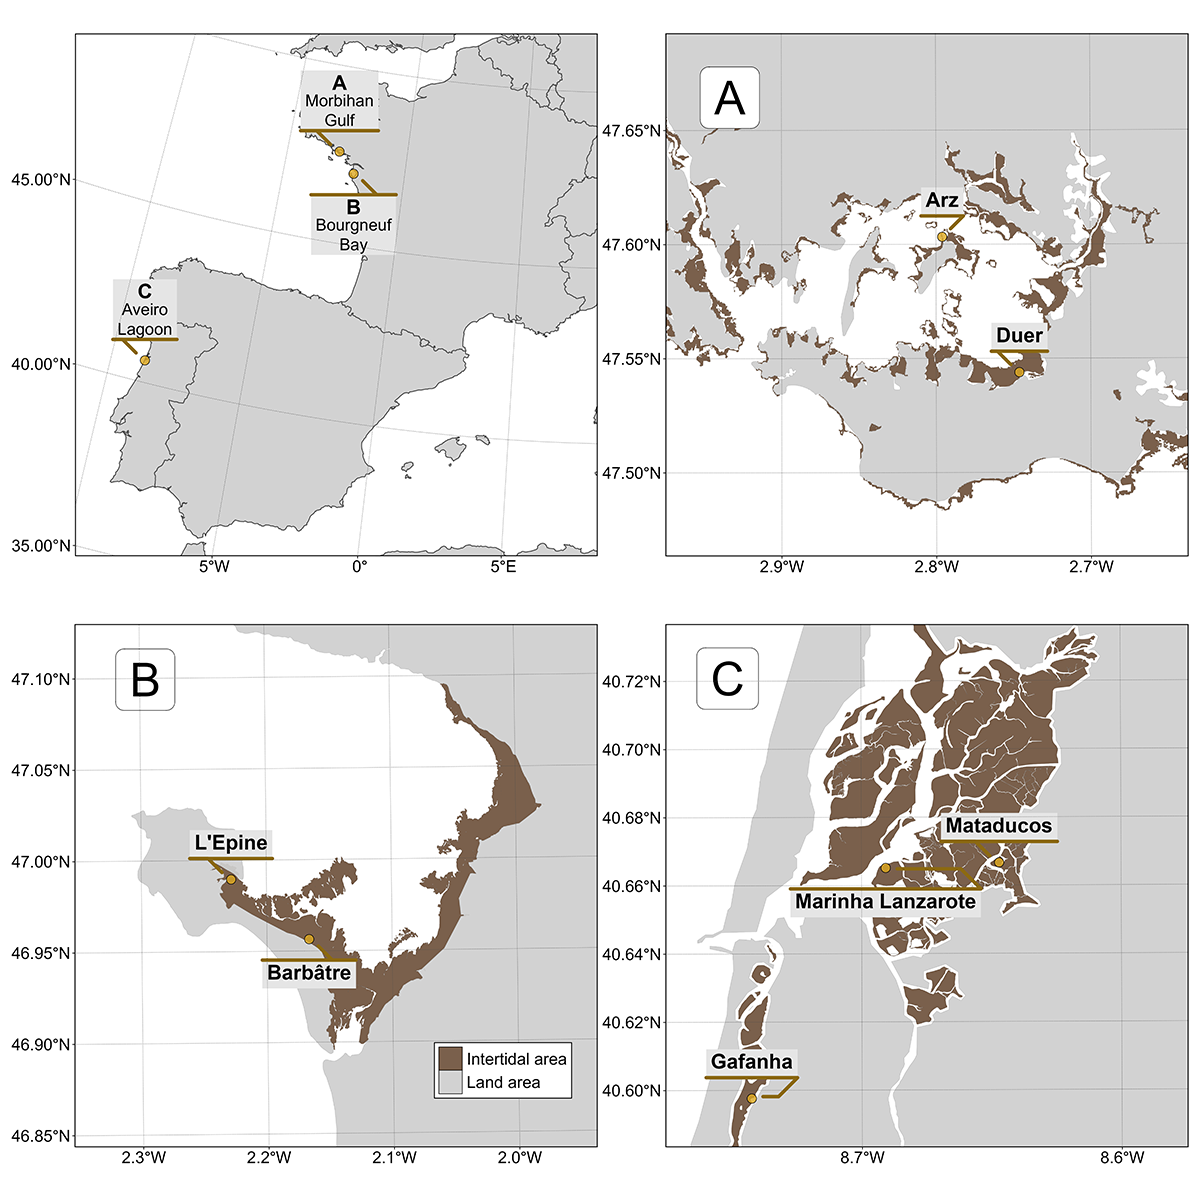
\includegraphics[width=1\textwidth,height=\textheight]{./Figures/Low_res/Fig1_Map_Drone_Sites.png}

}

\caption{\label{fig-map}Location of drone flights in France and
Portugal. A: Gulf of Morbihan (Two sites), B: Bourngeuf Bay (Two sites),
C: Ria de Aveiro Lagoon (Three sites). Green represent intertidal
areas.}

\end{figure}%

\subsection{Drone Data}\label{drone-data}

At each location, a DJI Matrice 200 quadcopter drone equipped with a
Micasense RedEdge Dual MX multispectral camera was flown to take 1.2
million pixel reflectance photographs in ten spectral bands, from 444 nm
(blue) to 840 nm (near infrared, NIR). An angle of 90° was maintained
between the sun and the drone's route to guarantee uniform lighting
conditions between flight lines. A side overlap of 70\% and a front
overlap of 80\% between each image was set for each flight. A
downwelling light sensor (DLS2) was used to acquire irradiance data
concomitantly with the camera measurements. Raw data were calibrated in
reflectance using a calibration panel reflective at \textasciitilde50\%
provided by the manufacturer. A structure-from-motion photogrammetry
software (Agisoft Metashape) was used to process images to obtain
multispectral orthomosaics of each flight. The workflow for
orthomosaicking was the same for every flight. First, tying key points
were detected inside of each image and between overlapping images in
order to obtain a sparse point cloud. This cloud was cleaned using
reprojection accuracy metric in order to remove noisy points. A dense
point cloud was then produced using a structure from motion algorithm. A
surface interpolation of this dense point cloud was made to obtain a
digital surface model (DSM), used to reconstruct the multispectral
ortho-image. Across all sites, flights were made at two different
altitudes : 12 m or/and 120 m. Low altitude drone flights produce
ortho-images with a very high spatial resolution (8 mm per pixel),
making it efficient to visually distinguish between the various types of
vegetation. High altitude fights on the other hand allow to cover large
areas and produced images with a pixel size of 80 mm
(Table~\ref{tbl-flights}).

\begin{table}

\caption{\label{tbl-flights}List of drone flight, summarising the date,
the altitude and the purpose of each flight. 12 m and 120 m flights have
a spatial resolution of 8 and 80 mm respectively.}

\centering{

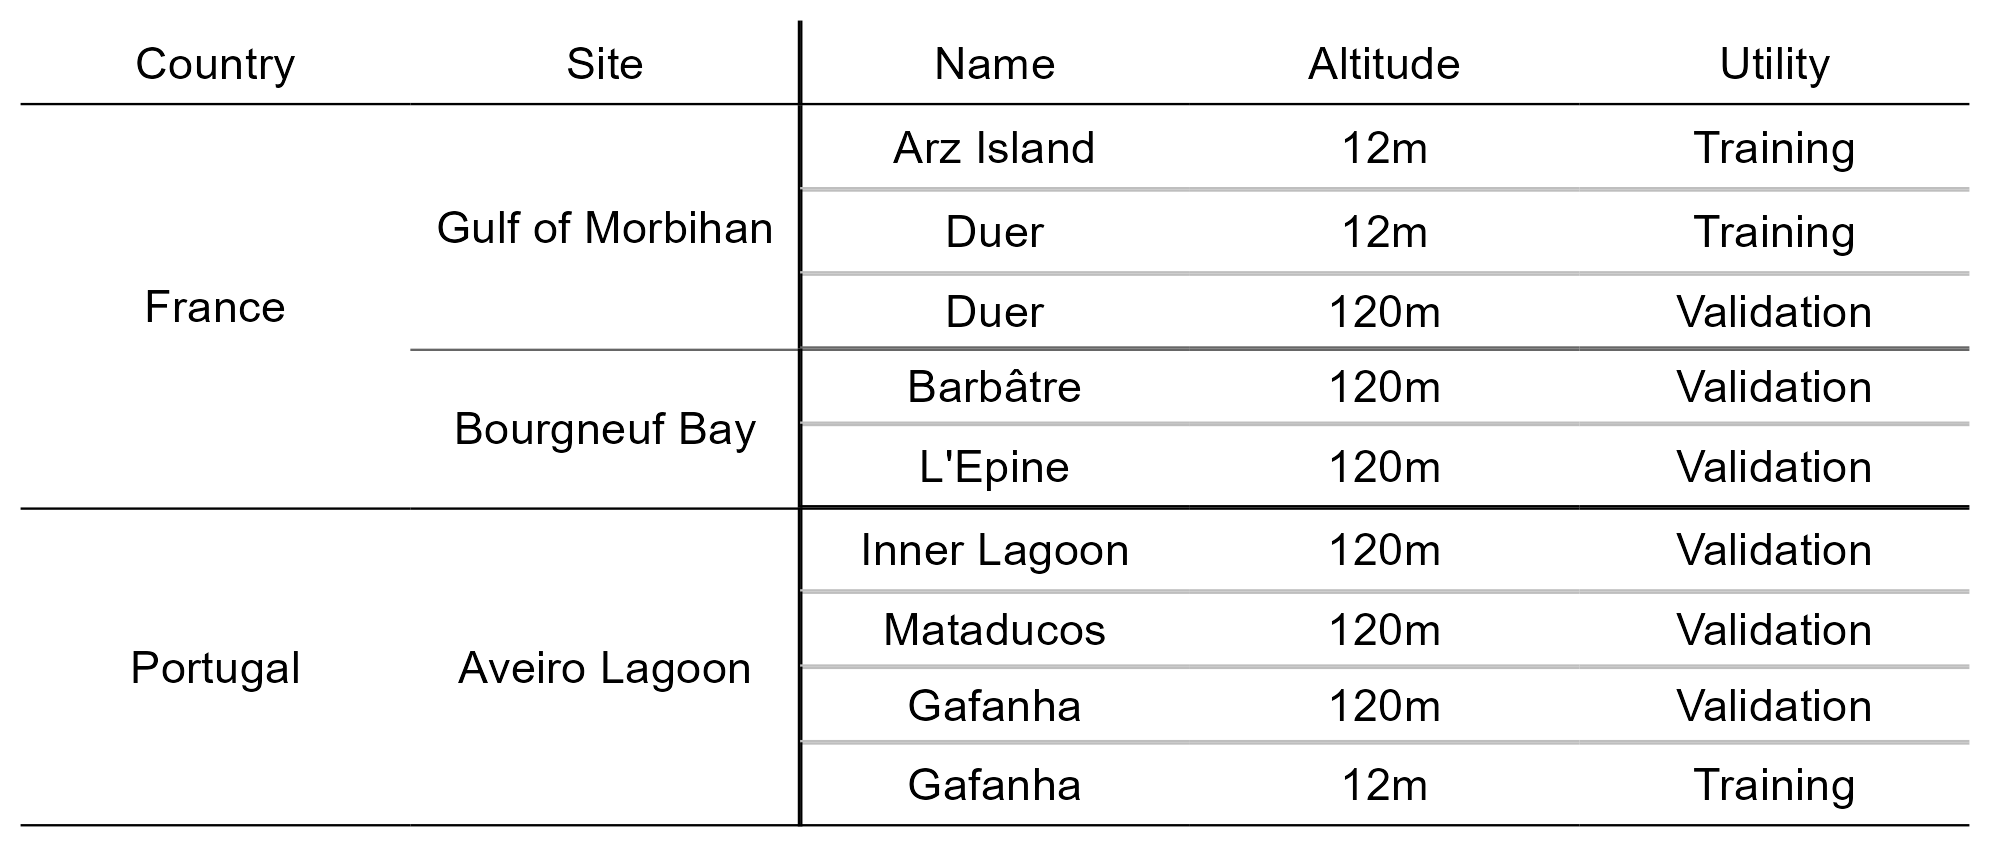
\includegraphics[width=6.63in,height=\textheight]{Figures/table_flights.png}

}

\end{table}%

\subsection{Field sampling}\label{field-sampling}

Before each flight, targets used as Ground Control Points (GCPs) were
distributed over the study site and georeferenced with a Trimble © Geo
XH 6000 differential GPS (dGPS). GCPs were used to correct
georeferencing imprecision of orthomosaics with an horizontal and
vertical accuracy of 10cm. dGPS was also used to georeference quadrats
of 0.25 m² assessing the presence or absence of five key taxonomic
classes of intertidal vegetation : Bacillariophyceae (Unicellular
benthic diatoms forming large biofilms at the sediment surface during
low tide), Phaeophyceae (brown macroalgae), Magnoliopsida (seagrass),
Chlorophyceae (green macroalgae) and Rhodophyceae (red macroalgae)
(Figure~\ref{fig-vegetation}). Pictures of each quadrat were uploaded
online on the Global Biodiversity Information Facility (GBIF) platform
\citep{BedeGbif}, a public open portal to store and share biodiversity
data. Each photograph was also processed to estimate the percent cover
of each type of vegetation using an image processing software (imageJ).
For all quadrats, the hyperspectral reflectance signatures of each
vegetation class was measured using an ASD FieldSpec HandHeld 2
spectroradiometer, which acquires reflectance between 325 and 1075 nm,
with 1 nm of spectral resolution. Hyperspectral signatures from quadrats
serve dual purposes: they validate the radiometric calibration of drone
data and contribute to error reduction in photo interpretation. The
workflow developped in this study is presented in
Figure~\ref{fig-workflow}.

\phantomsection\label{cell-fig-vegetation}
\begin{figure}[H]

\centering{

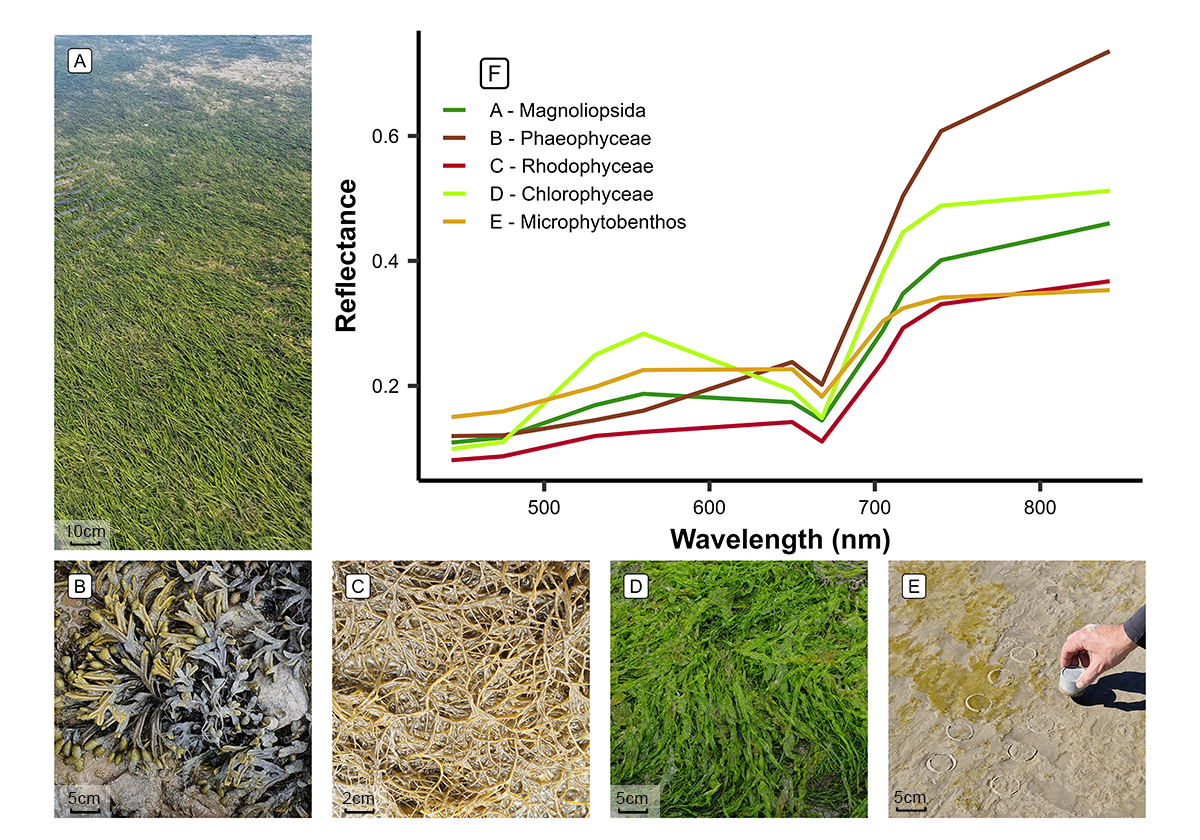
\includegraphics[width=1\textwidth,height=\textheight]{Figures/Low_res/Spectral_shapes_total.png}

}

\caption{\label{fig-vegetation}The five taxonomic classes of vegetation
used to train the Neural Network model and their raw spectral signatures
at the spectral resolution of the Micasense RedEdge Dual MX.}

\end{figure}%

\subsection{Intertidal vegetation
mapping}\label{intertidal-vegetation-mapping}

\phantomsection\label{cell-fig-workflow}
\begin{figure}[H]

\centering{

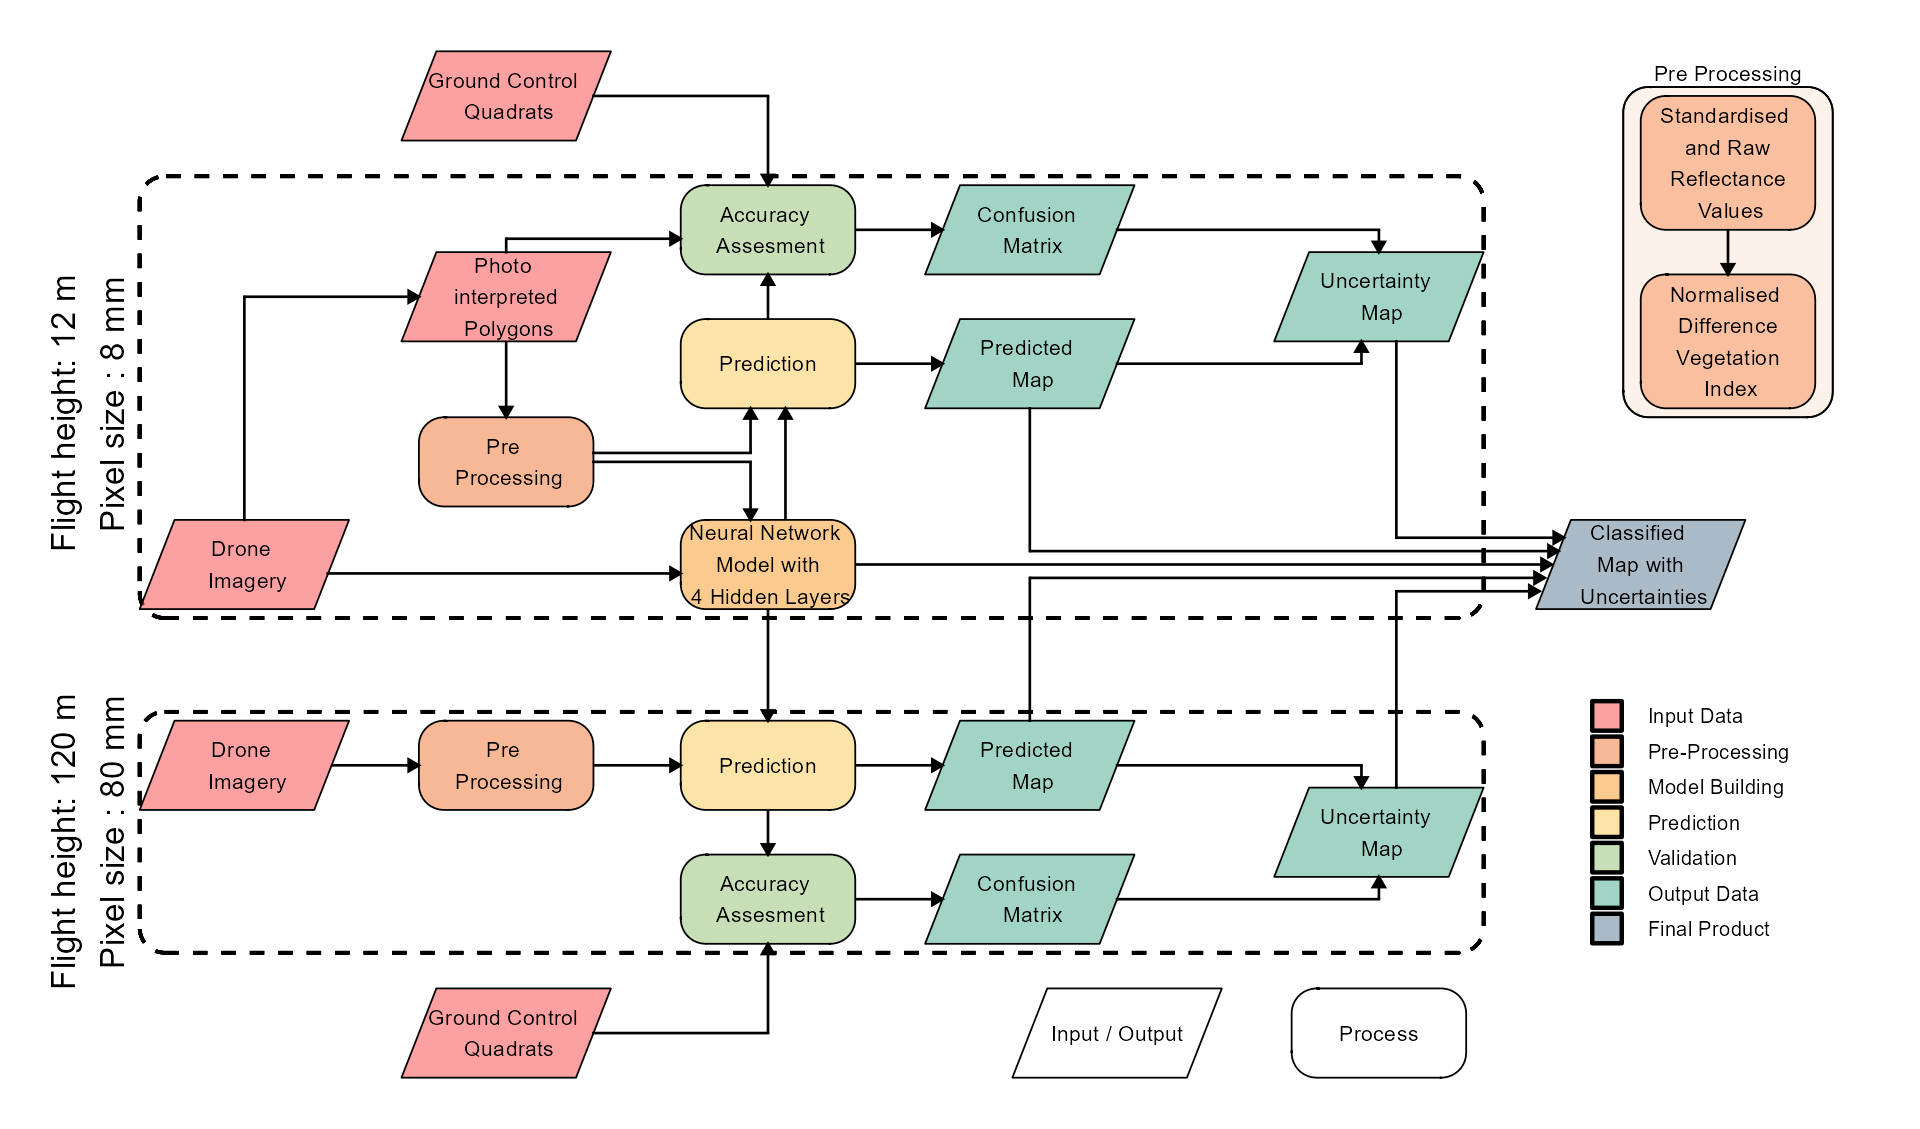
\includegraphics[width=1\textwidth,height=\textheight]{./Figures/Low_res/Figure3_workflow.png}

}

\caption{\label{fig-workflow}Schematic representation of the workflow.
Diamonds represent input or output data, and rectangles represent Python
processing algorithms. The overall workflow of this study is divided
into two distinct parts based on the spatial resolution of the drone
flights: high-resolution flights (pixel size: 8 mm) were utilized for
training and prediction of the Neural Network model, whereas
lower-resolution flights (pixel size: 80 mm) were solely employed for
prediction purposes. Validation has been performed on both high and low
resolution flights.}

\end{figure}%

The spectral similarities of the reflectance signatures between
intertidal green macrophytes (Magnoliopsida and Chlorophyceae) make
their discrimination challenging using simple classification algorithms
(Figure~\ref{fig-vegetation} F). To overcome this challenge, a deep
learning classification method was developed, trained, validated, and
applied to each drone flight (Figure~\ref{fig-workflow}).

\subsubsection{Neural Network model
building}\label{neural-network-model-building}

\begin{table}

\caption{\label{tbl-validationPX}Vegetation Classes of the model and the
number of pixels used to train and validate each class}

\centering{

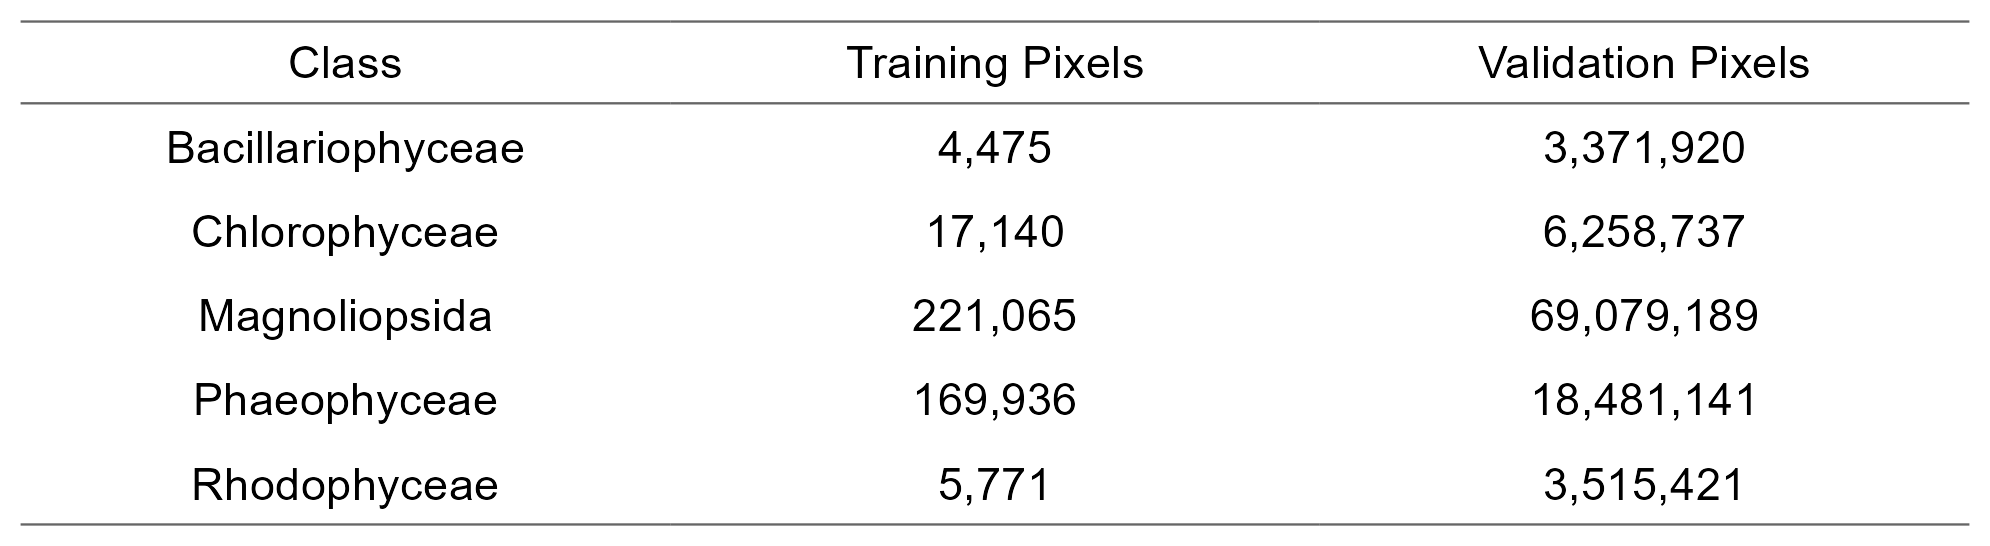
\includegraphics[width=6.63in,height=\textheight]{Figures/table_validation_px.png}

}

\end{table}%

A dataset containing photo-interpreted drone reflectance pixels was
built to train a Neural Network model with 2 hidden layers. The training
pixels were categorized into seven different classes, representing the
various habitats encountered at the different study sites: Sediment,
Water, Chlorophyceae, Magnoliopsida, Bacillariophyceae, Phaeophyceae and
Rhodophyceae. Only low-altitude flights (Table~\ref{tbl-flights}) were
used for training because their 8 mm spatial resolution allowied to
avoid spectral sub-pixel mixing and to accurately differentiate
vegetation classes. More than 418,000 pixels at 8 mm resolution from the
3 training flights were used to train the model
(Table~\ref{tbl-validationPX}). Twenty one variables were used by the
model as predictors: the ten raw spectral bands of the Micasense RedEdge
Dual MX multispectral camera (ranging from 444 nm to 840 nm), the same
ten spectral bands standardized using a min/max transformation
(Equation~\ref{eq-std} ; \citep{Cao2017}) and the Normalized difference
vegetation index (NDVI, Equation~\ref{eq-ndvi}). Standardisation of
spectral bands is used to eliminate the scaling differences between
spectra and to limit the effect of biomass on the shape of the spectra
\citetext{\citealp[ ]{Douay2022}; \citealp{Davies2023}}.

\begin{equation}\phantomsection\label{eq-std}{
R_{i}^{*}(\lambda) = \frac{R_{i}(\lambda) - min(R_{i})}{max(R_{i})- min(R_{i})}
}\end{equation}

where \(R_{i}(\lambda)\) is the reflectance at the wavelength
\((\lambda)\) of each individual spectra \((i)\), \(min(R_{i})\), and
\(max(R_{i})\) are the minimum and maximum value of the spectra \((i)\)

\begin{equation}\phantomsection\label{eq-ndvi}{
NDVI = \frac{R(840nm)-R(668nm)}{R(840nm)+R(668nm)}
}\end{equation}

where \(R(840nm)\) is the reflectance at 840 nm and \(R(668nm)\) is the
reflectance at 668 nm.

\subsubsection{Validation}\label{validation}

The workflow of this study revolves around two distinct flight heights
(12 m and 120 m, Figure~\ref{fig-workflow}) where ensuring consistency
between reflectances at both heights is crucial. This comparison was
conducted at sites where low and high altitude flights overlapped. The
low altitude flights were resampled to the same spatial resolution and
grid as the high flights using a median resampling method. Reflectance
values were then extracted, and a scatterplot was generated.
Subsequently, the slope of the linear model and the coefficient of
determination (R²) were computed.

The model was applied to all flights at both 12 and 120 m of altitude.
In situ information on georeferenced class type and percent cover
collected during each flight was used to assess the model accuracy.
These images were used to construct a validation dataset indicating the
presence or absence of each class. Additionally to the quadrat-based
validation dataset, polygons of each class were photo interpreted in
order to increase the number of pixels of the validation dataset. A
confusion matrix, along with precision metrics such as global accuracy,
sensitivity, specificity, and Kappa coefficient, was generated for each
sites. All validation matrices were then merged to create a unique
matrix . Altogether, a total of 536,000 pixels was used to validate the
model, thus providing a geographically robust validation dataset.

\section{Results}\label{results}

\subsection{Classification}\label{classification}

A total of 9 prediction maps corresponding to the 9 drone flights were
obtained. Each prediction map is associated with a probability map,
indicating the probability of the selected class for every pixel. The
low-altitude flight conducted in Gafanaha, Portugal, represents the site
with the highest complexity (Figure~\ref{fig-GafLow}). Among the 5
vegetation classes on which the model was trained, 4 were present on
this site. On this site, there is a mixture of Chlorophyceae and
Rhodophyceae over the seagrass meadow. This is also where
Bacillariophyceae is most abundant. Although the seagrass bed is solely
composed of \emph{Zostera noltei}, various colors can be observed: dark
green (indicating healthy beds with 100\% coverage) and whitish/brown
(indicating beds where leaves are dying). Regardless of the color, the
meadow is predicted as Magnoliopsida by the model.

\phantomsection\label{cell-fig-GafLow}
\begin{figure}[H]

\centering{

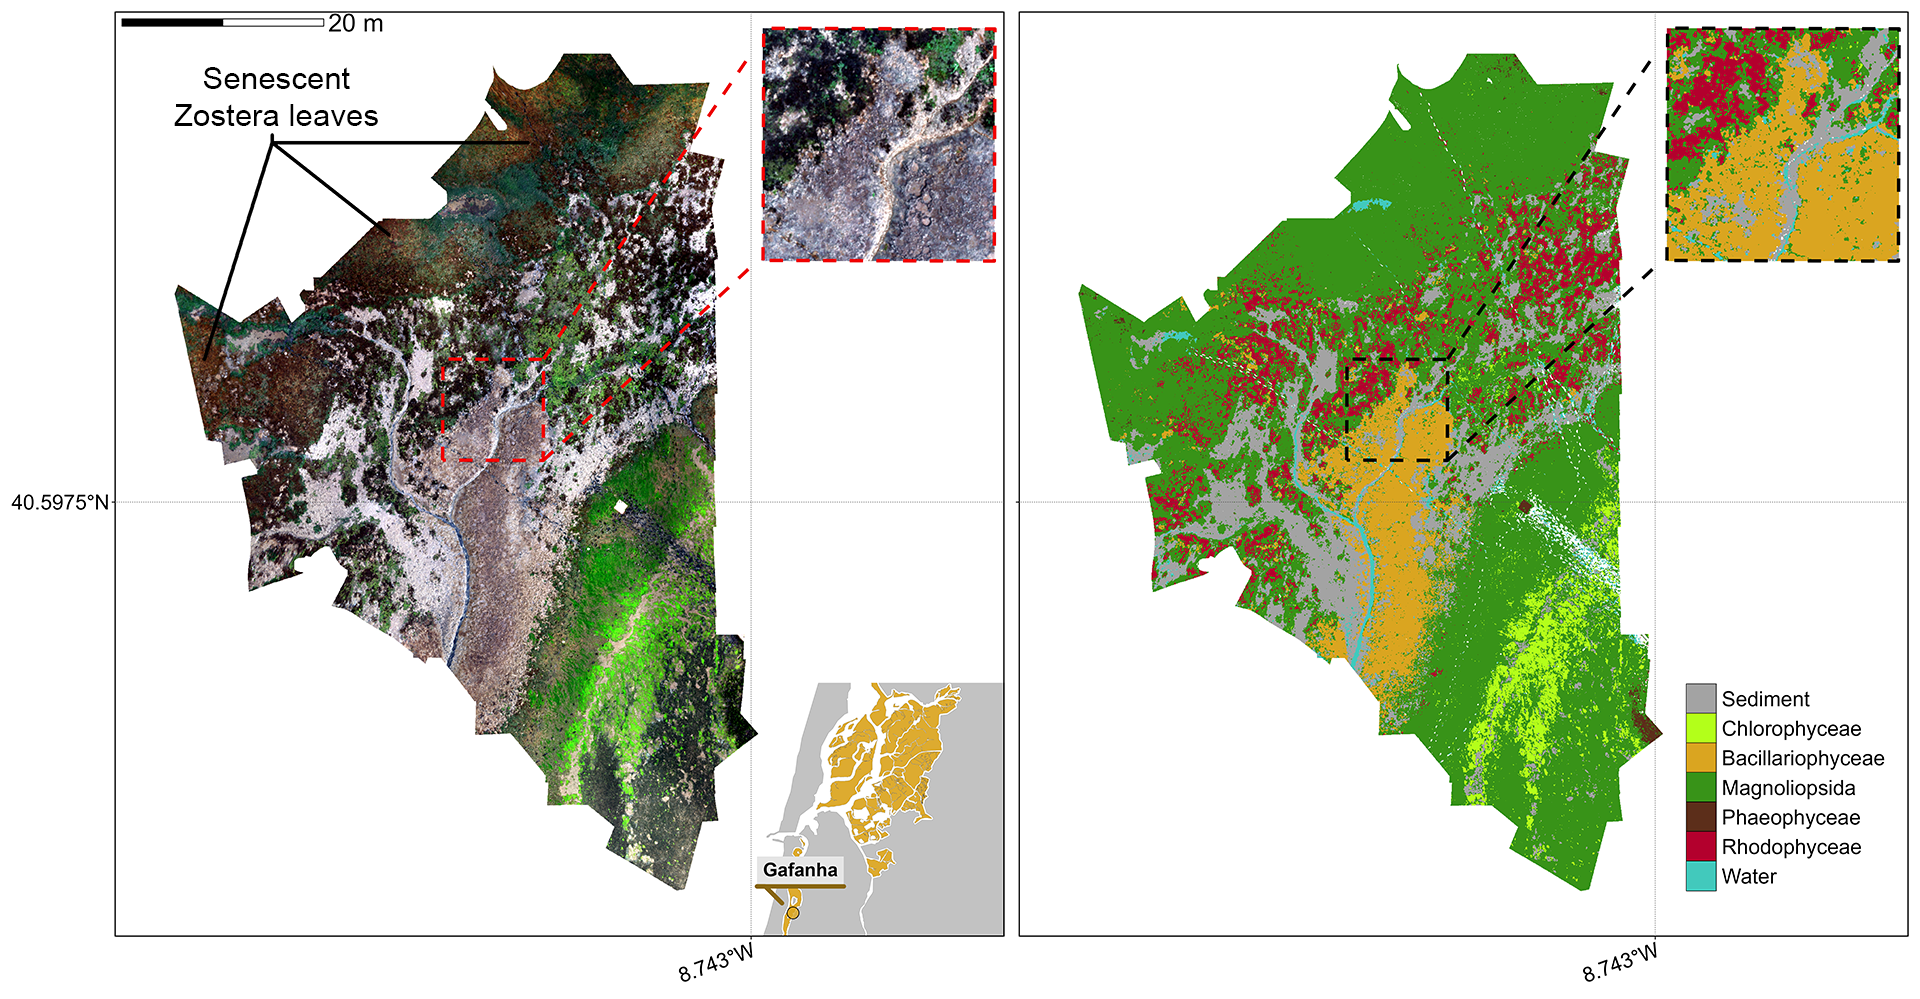
\includegraphics[width=1\textwidth,height=\textheight]{./Figures/Low_res/Maps Pred/FigX-Gaf_Low_Pred.png}

}

\caption{\label{fig-GafLow}RGB orthomosaic (Left) and Prediction (Right)
of the low altitude flight of Gafanaha, Portugal. The total extent of
this flight is 3000m² with a resolution of 8 mm per pixel. Background
colors means intertidal area (Light Green) and land area (Light Grey).
The zoom covers an area equivalent to a 10-meter Sentinel-2 pixel size.}

\end{figure}%

The high-altitude flight over Gafanha covered nearly 1 km² in total
(Figure~\ref{fig-GafHigh}). A channel delineating a small island was
masked in the prediction map due to sunglint and misclassification
caused by the turbid shallow water. Most of the intertidal area has been
classified as Magnoliopsida by the model, even though there is
discoloration of seagrass blades. Only a few pixels have been classified
as Chlorophyceae at this scale. Furthermore, the area that was
classified as Bacillariophyceae in the low-altitude flight remains
mostly classified as such in the high-altitude flight, though some
pixels were classified as Magnoliopsida. Patches of Rhodophyceae were
correctly classified. In the nothern part of the scene, near the land
limit, patches of \emph{Spartina sp.} were misclassified, either as
Magnoliopsida or as Phaeophyceae.

\phantomsection\label{cell-fig-GafHigh}
\begin{figure}[H]

\centering{

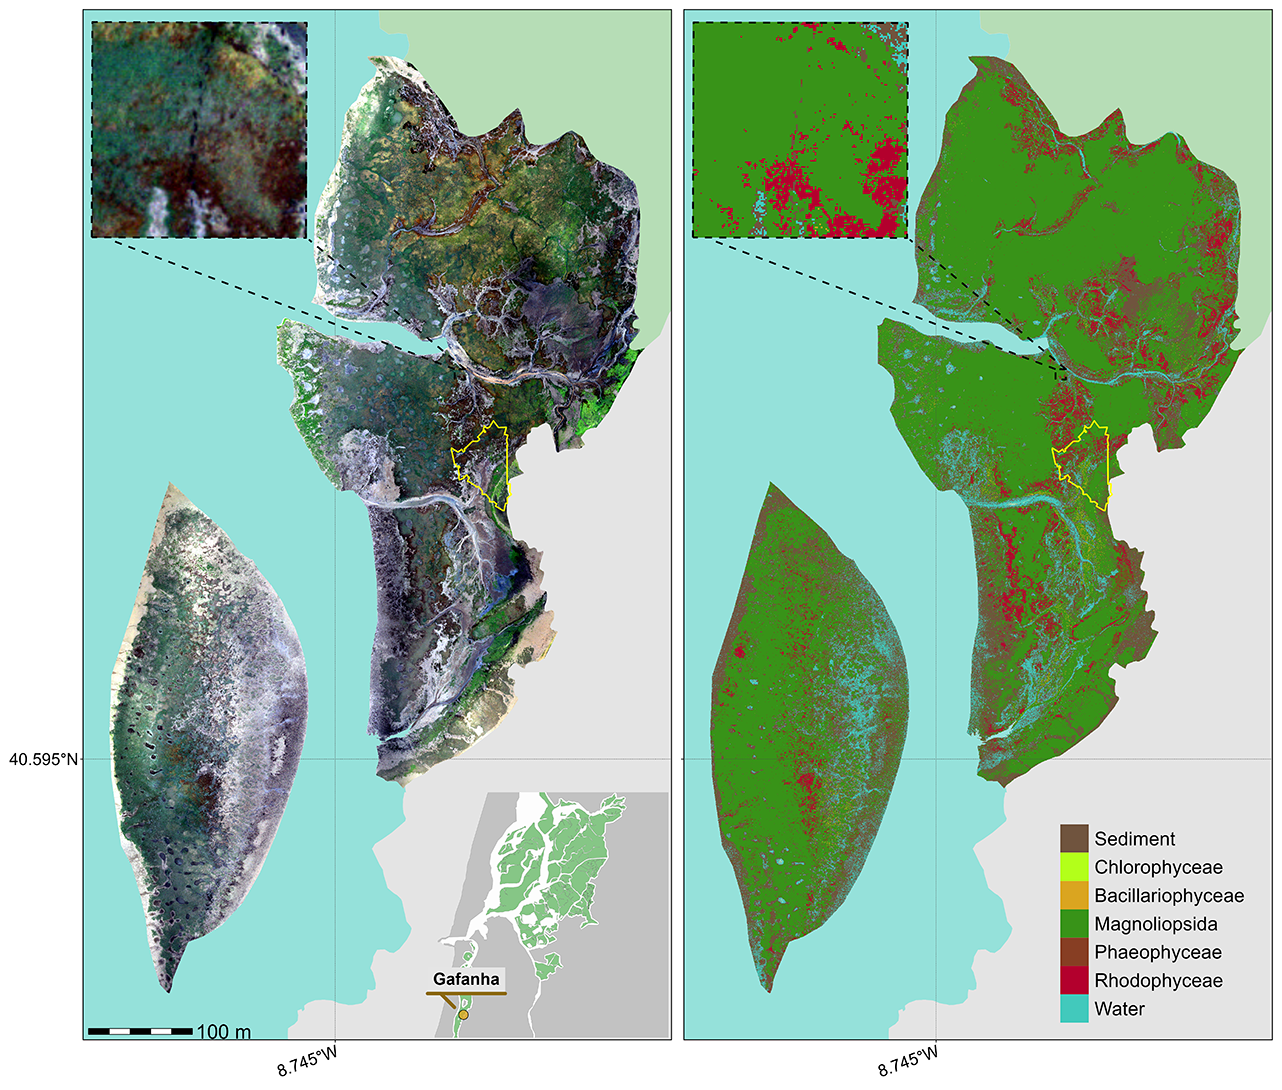
\includegraphics[width=1\textwidth,height=\textheight]{./Figures/Low_res/Maps Pred/FigX-Gaf_High_Pred.png}

}

\caption{\label{fig-GafHigh}RGB orthomosaic (Left) and Prediction
(Right) of the high altitude flight of Gafanaha, Portugal. The total
extent of this flight is about 1 km² with a resolution of 80 mm per
pixel. Background colors means intertidal area (Light Green), land area
(Light Grey) and water (Light Blue). The red triangle shows the extent
of the low altitude flight of Gafanha. The zoom covers an area
equivalent to a 10-meter Sentinel-2 pixel size.}

\end{figure}%

The high altitude flight acquired over the inner lagoon of the Ria de
Aveiro is the largest of all flights, covering almost 1.5 km²
(Figure~\ref{fig-Boat}). On this site, only seagrass and red algae where
seen on the field. The classification provided consistent results, with
a patchy Magnoliopsida meadow mixed with Rhodophyceae on the eastern
part of the scene. As shown in the zoom (Figure~\ref{fig-Boat}), the
edges of the meadow can be colonised by Chlorophyceae.

\phantomsection\label{cell-fig-Boat}
\begin{figure}[H]

\centering{

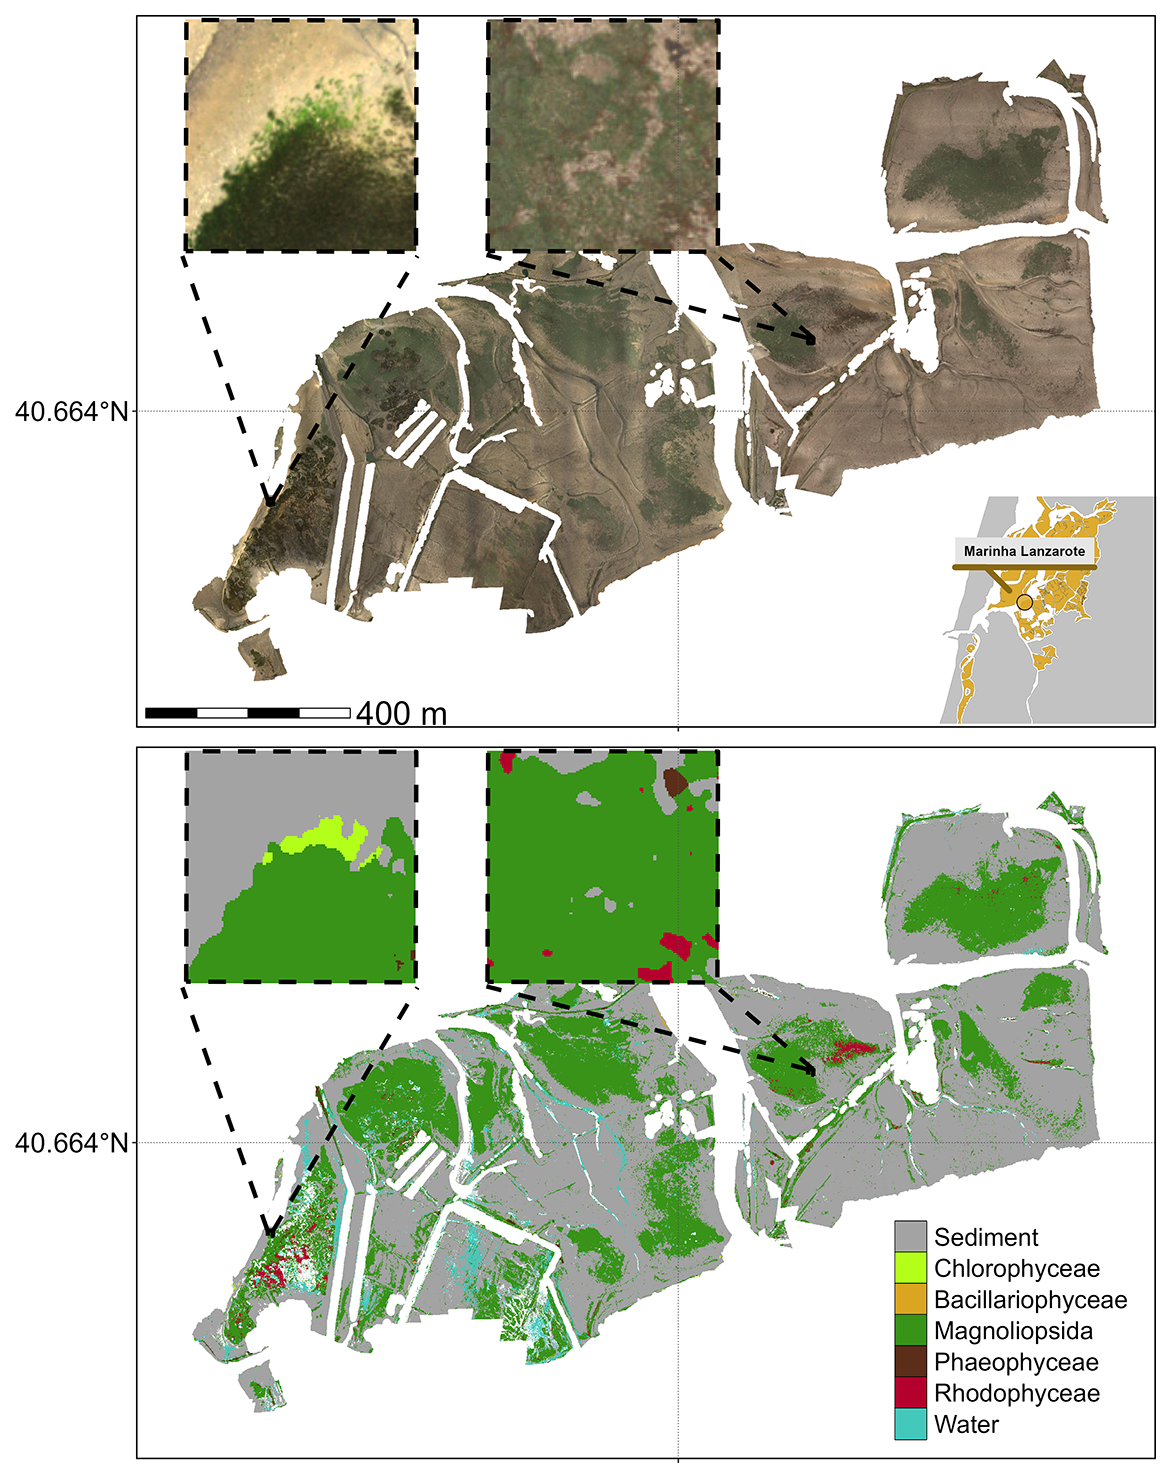
\includegraphics[width=1\textwidth,height=\textheight]{./Figures/Low_res/Maps Pred/FigX-Boat_Pred.png}

}

\caption{\label{fig-Boat}RGB orthomosaic (Top) and Prediction (Bottom)
of the flight made in the inner part of Ria de Aveiro Lagoon, Portugal.
The total extent of this flight is about 1.5 km² with a resolution of 80
mm per pixel. Background colors means intertidal area (Light Green),
land area (Light Grey) and water (Light Blue). The zoom covers an area
equivalent to a 10-meter Sentinel-2 pixel size.}

\end{figure}%

The flight over L'Epine in Noirmoutier Island, France
(Figure~\ref{fig-Dike}) was conducted near a dike crossing the northern
part of the scene from west to east. Alongside this dike, brown algae
attached to rocks and stranded green algae could be found. Despite the
high mixture between Chlorophyceae and Magnoliopsida these two classes
were correctly discriminated by the classifier.

\phantomsection\label{cell-fig-Dike}
\begin{figure}[H]

\centering{

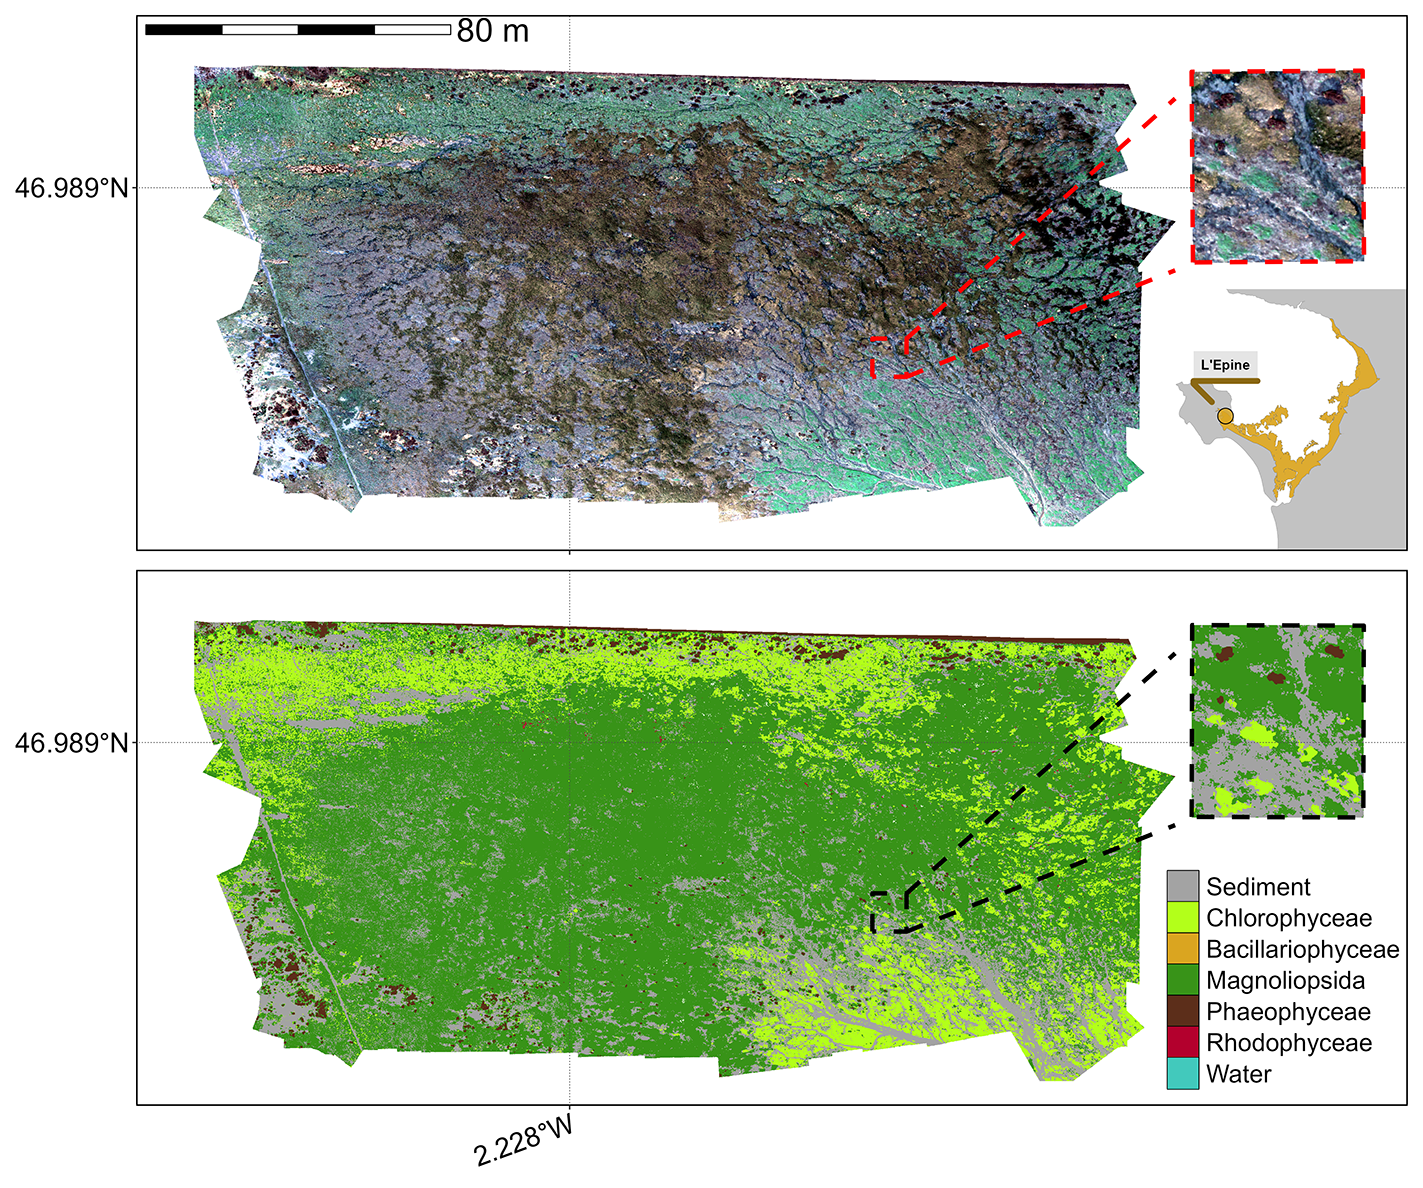
\includegraphics[width=1\textwidth,height=\textheight]{./Figures/Low_res/Maps Pred/FigX-Dike_Pred.png}

}

\caption{\label{fig-Dike}RGB orthomosaic (Top) and Prediction (Bottom)
of Northern part of Noirmoutier Island, France. The total extent of this
flight is about 28 000 m² with a resolution of 80 mm per pixel.
Background colors means intertidal area (Light Green) and land area
(Light Grey). The zoom covers an area equivalent to a 10-meter
Sentinel-2 pixel size.}

\end{figure}%

\subsection{Validation}\label{validation-1}

\phantomsection\label{cell-fig-Validation}
\begin{figure}[H]

\centering{

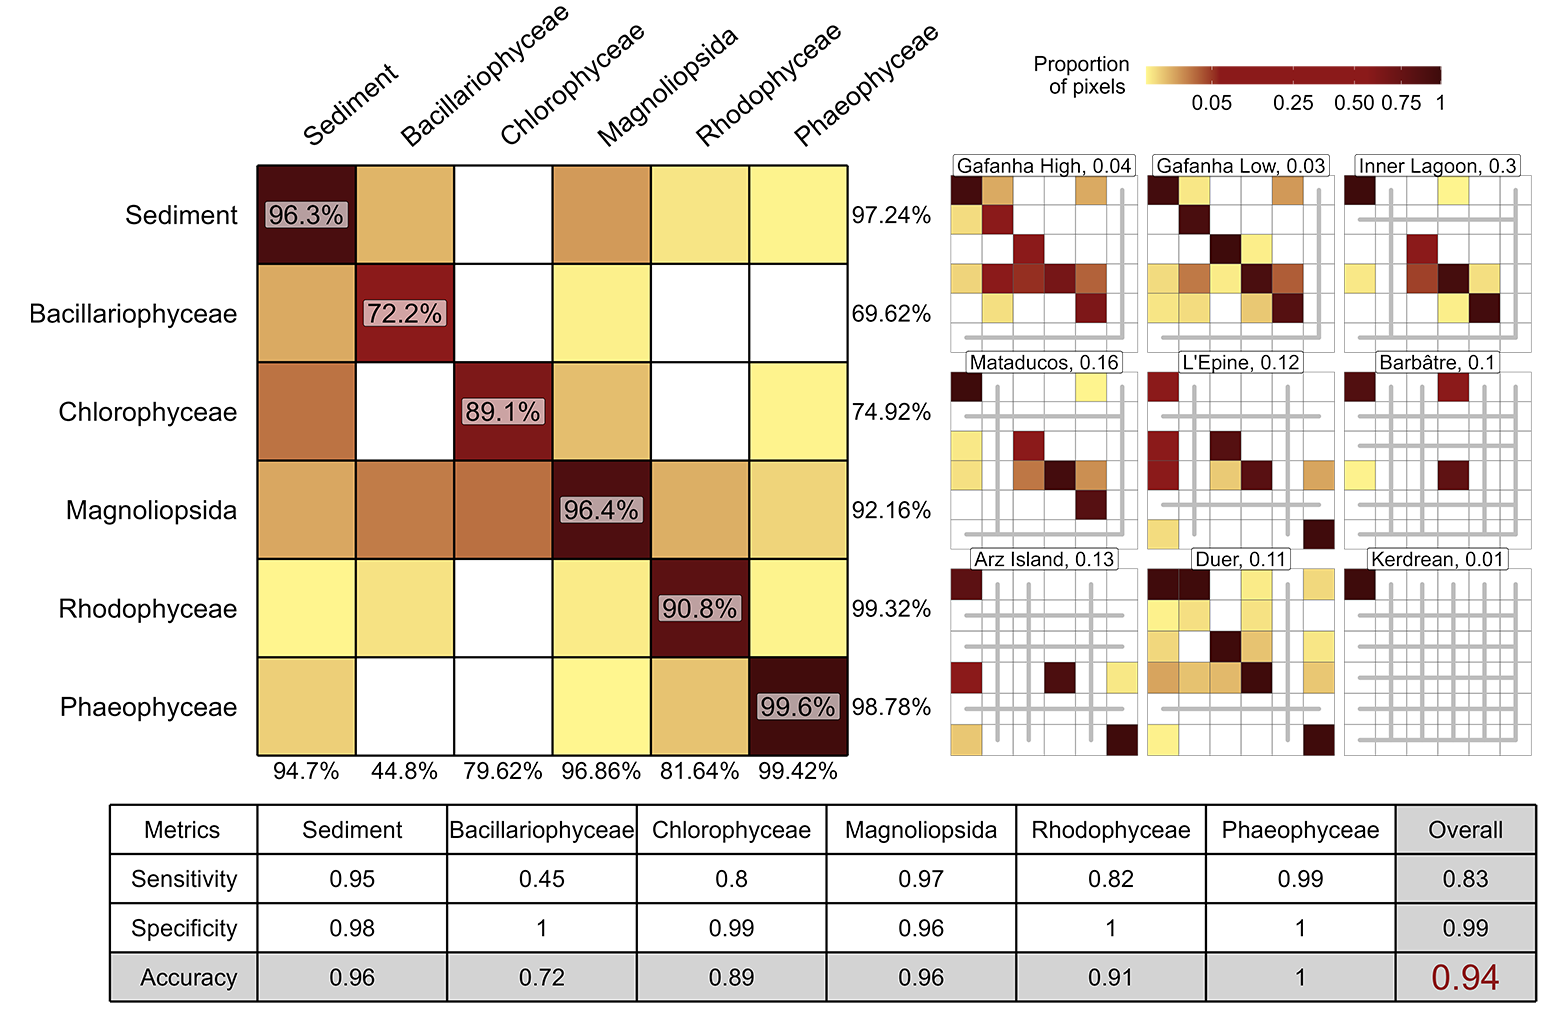
\includegraphics[width=1\textwidth,height=\textheight]{./Figures/Low_res/Validation/ConfusionMatrixGlobal.png}

}

\caption{\label{fig-Validation}A global confusion matrix on the left is
derived from validation data across each flight, while a mosaic of
confusion matrices from individual flights is presented on the right.
The labels inside the matrices indicate the balanced accuracy for each
class. The labels at the bottom of the matrices indicate the User's
accuracy for each class, and those on the right indicate the Producer's
Accuracy. The values adjacent to the names of each site represent the
proportion of total pixels from that site contributing to the overall
matrix. Grey lines within the mosaic indicate the absence of validation
data for the class at that site. The table at the bottom summarizes the
Sensitivity, Specificity, and Accuracy for each class and for the
overall model.}

\end{figure}%

A total of 536,000 pixels was used to validate the Neural Network
classifier. The sites with the lowest and highest number of validation
data were Kerdrean (5557 pixels) and Marinha Lanzarote (159713 pixels),
respectively. Model global accuracy was 94.26\% with a Kappa coefficient
of 0.92 (Figure~\ref{fig-Validation}). The least performing site was
Gafanha High (global accuracy of 75.45\%) whereas Mataducos was the site
with the most accurate prediction (global accuracy of 98.05\%). Overall,
the classes Phaeophyceae, Magnoliopsida, Sediment and Rhodophyceae were
correctly classified with a balanced accuracy of 1, 0.96, 0.96 and 0.91
respectively. Bacillariophyceae was the least performing class (accuracy
of 0.72 ) mainly due to the confusion between Magnoliopsida and
Sediment.

\subsection{Variable importance}\label{variable-importance}

\phantomsection\label{cell-fig-VIP}
\begin{figure}[H]

\centering{

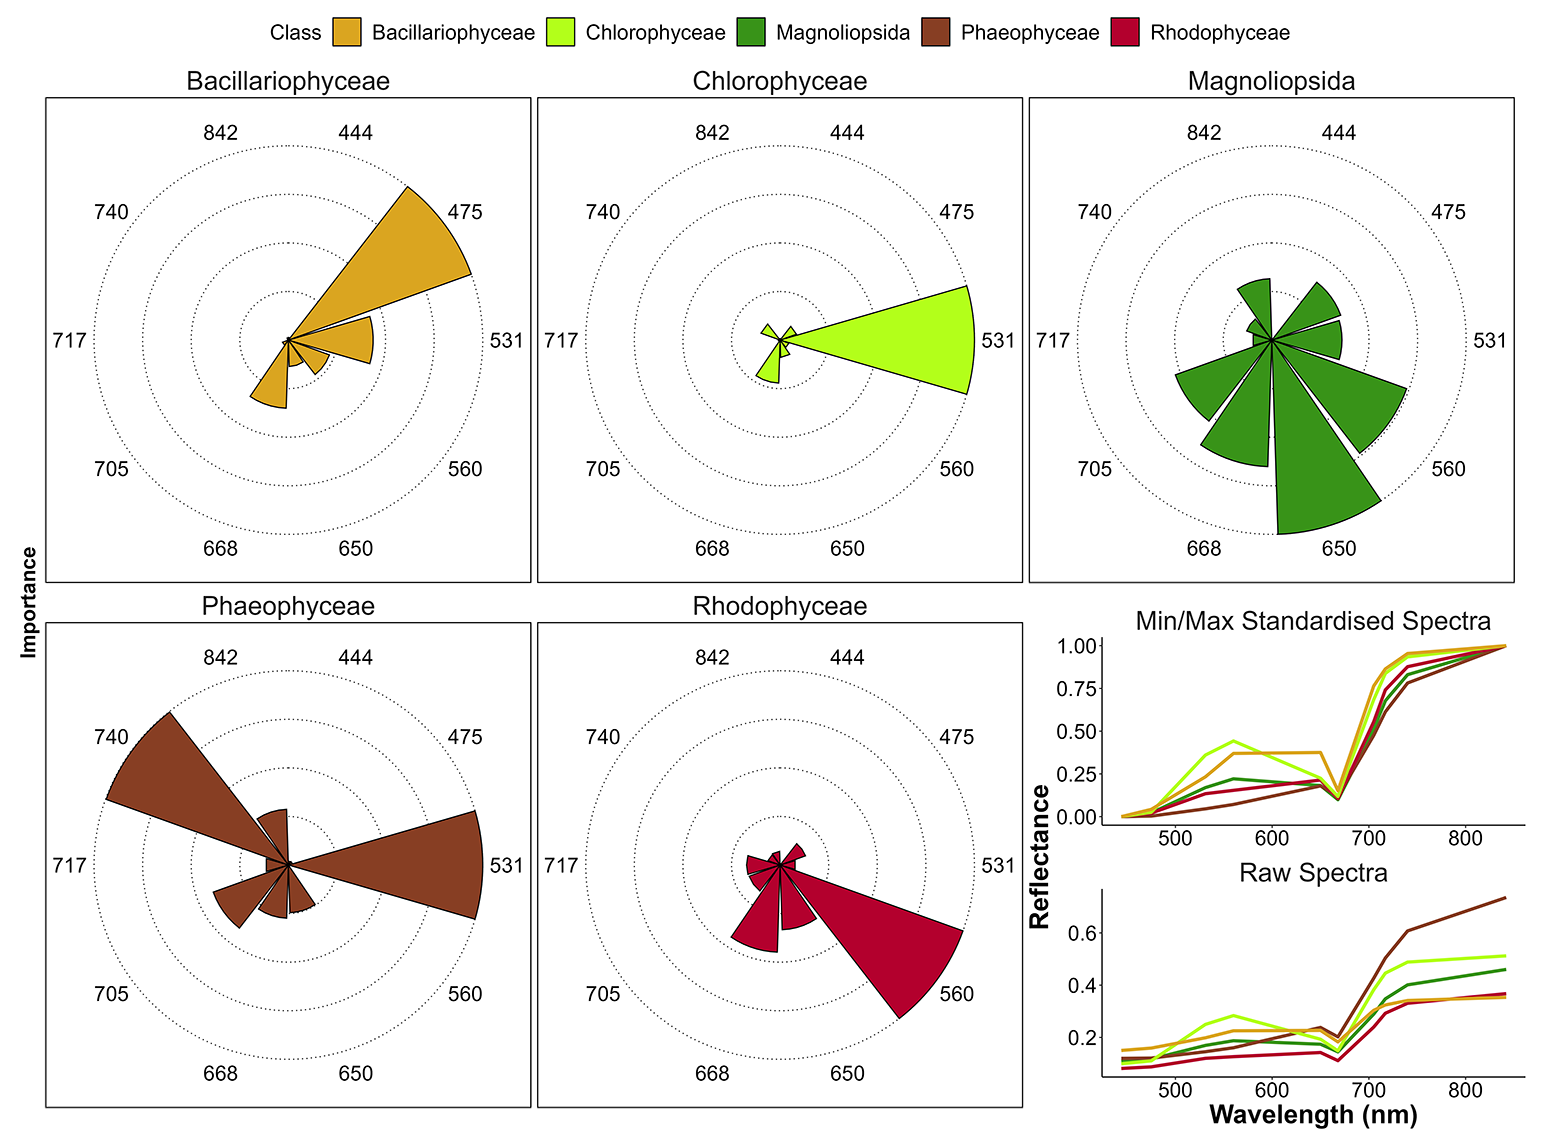
\includegraphics[width=1\textwidth,height=\textheight]{Figures/Low_res/VIP/Fig_VIP.png}

}

\caption{\label{fig-VIP}Variable Importance of the Neural Network
Classifier for each vegetation class. The bigger the slice, the more
important is the variable to predict accuratly this class. The bottom
right plot shows the drone standardised reflectance spectra of each
class. Each slice represent the VIP of both RAW and standardised
reflectance combined.}

\end{figure}%

The computation of the variable importance makes it possible to identify
which wavelengths are the most useful for class prediction
(Figure~\ref{fig-VIP}). The spectral bands at 444 , 717 and 842 nm of
the Micasense camera are important for none of the vegetation classes.
The band at 531 nm is the only important predictor for the classifier to
accurately predict chlorophyceae. In fact, at this wavelength, the
Chlorophyceae spectra has the maximum reflectance among of all
vegetation classes. The bands at 531 and 740 nm are the most important
predictors for Phaeophyceae, corresponding to the minimum reflectance
among all classes. Bands at 475 and 560 nm are the most important
predictors for Bacillariophyceae and Rhodophyceae, respectively. Four
predictors, ranging from the green (560 nm) to the RedEdge (705 nm)
bands are important to accurately predict magnoliopsida.

\subsection{Effect of the flight height on the
prediction}\label{effect-of-the-flight-height-on-the-prediction}

\phantomsection\label{cell-fig-upscaling}
\begin{figure}[H]

\centering{

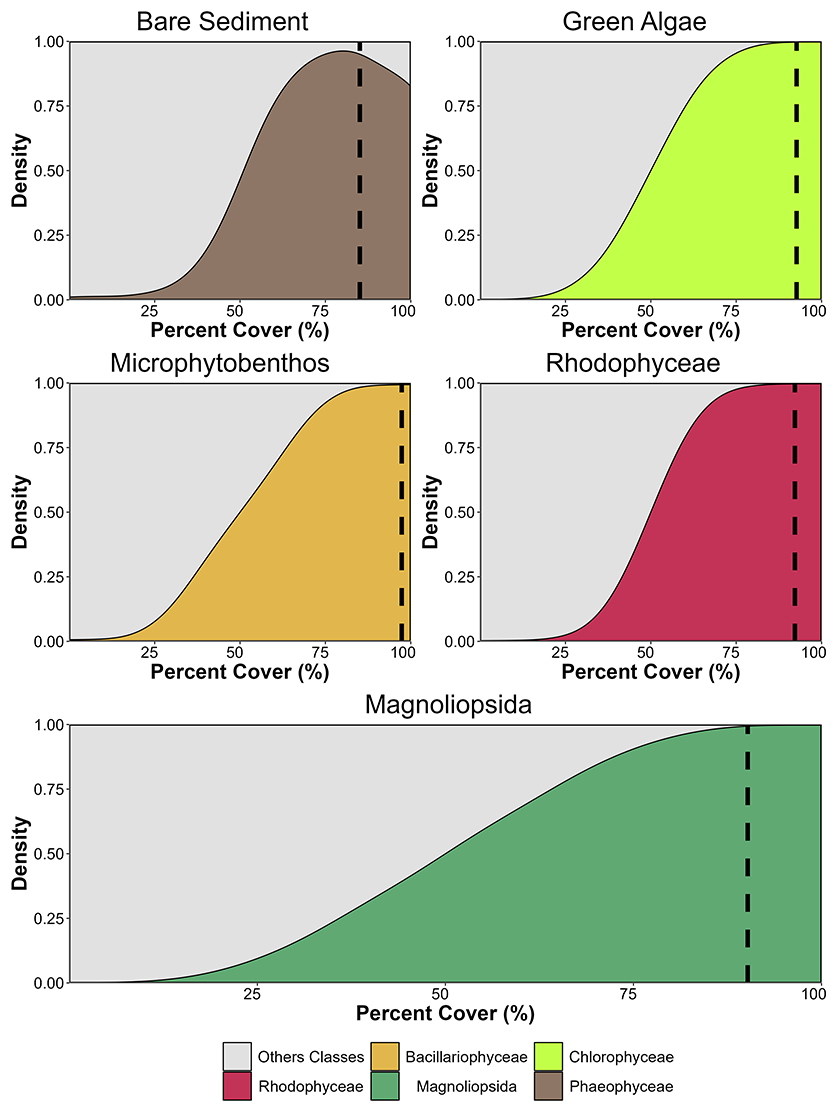
\includegraphics[width=0.9\textwidth,height=\textheight]{Figures/Low_res/Upscaling/density_vs_Proportion.png}

}

\caption{\label{fig-upscaling}Kernel density plot showing the proportion
of pixel well classified based on the percent cover of the class in high
altitude flight pixels of Gafanha, Portugal. Each subplot shows all the
pixels of the same classes on the hight altitude flight. Percent cover
of classes is retrieve using the result of the classification of the low
altitude flight of Gafanha, Portugal. The vertical dashed line shows the
0.85 probability of the model. Everything on the right of this line has
a probability higher then 0.85 and everuthing on the left of this line
has a probability lower.}

\end{figure}%

Using the very high precision low altitude flight, we determined the
minimal percent cover required to classify correctly classify a given
class using the high altitude flight (Figure~\ref{fig-upscaling}). When
the percent cover of the class is 100 \%, big pixels are well classified
for all the classes excepted for Bare Sediment, where it's well
classified 80\% of the time. A vegetative percent cover of at least 80\%
is need to have all the big pixels well classified, at the exception of
Magnoliopsida that needs an higher percent cover (\textgreater90 \%) to
be well classified. Concerning the probability of each class, a really
high Percent cover is needed to confidently predict Bacillariophyceae.
To predict Chlorophyceae with a confidence of 0.85, a percent cover of
93 \% is needed, 90 \% for magnoliopsida, 92 \% for Rhodophyceae and 97
\% for Bacillariophyceae.

\section{Discussion}\label{discussion}

\subsection{Vegetation Discrimination}\label{vegetation-discrimination}

\phantomsection\label{cell-fig-Pigm}
\begin{figure}[H]

\centering{

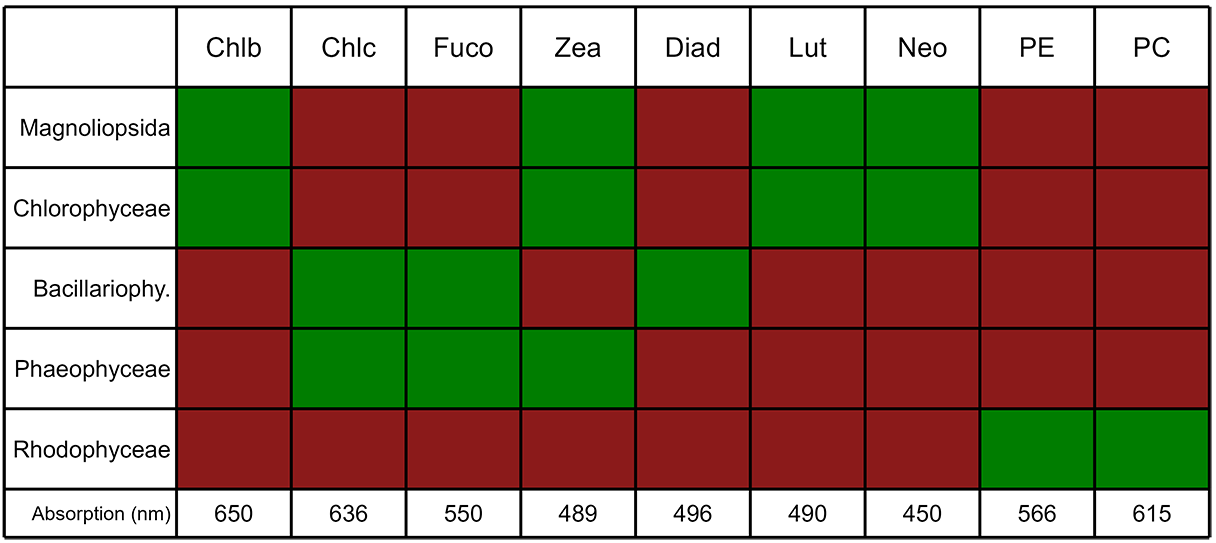
\includegraphics[width=1\textwidth,height=\textheight]{./Figures/Low_res/Disc_Pigment_Table.png}

}

\caption{\label{fig-Pigm}Photosynthetic and carotenoid pigments present
(Green) or absent (Red) in each taxonomic class present in the Neural
Network Classifier, along with their absorption wavelength measured with
spectroradiometer. Chl b: chlorophyll b, Chl c: chlorophyll c, Fuco:
fucoxanthin, Zea: zeaxanthin, Diato: diatoxanthin, Diadino:
diadinoxanthin, Neo: neoxanthin.}

\end{figure}%

The primary objective of this study was to develop a method for the
accurate classification of macrophytes on intertidal mudflats,
specifically focusing on distinguishing between Chlorophyceae (green
algae) and marine Magnoliopsida (seagrasses) using multispectral drone
data. The ability to differentiate between various types of vegetation,
as demonstrated in this study, plays a critical role in ecological
monitoring and management. By distinguishing between seagrasses and
macroalgae, our approach facilitates targeted conservation strategies,
enabling more effective preservation and restoration efforts in coastal
ecosystems. The discrimination of seagrasses from green macroalgae
presents significant challenges, primarily due to the shared pigment
composition between these taxa, as depicted in Figure~\ref{fig-Pigm} but
also by the frequent spatial mixing of these green macrophytes. This
similarity in pigment composition, including photosynthetic and
carotenoid pigments like chlorophyll b and c, fucoxanthin, and
neoxanthin, results in spectral signatures that are often
indistinguishable to non exper eyes. This spectral overlap is further
complicated by the intermingling of seagrasses and green macroalgae in
the same spatial locations, posing a significant challenge for remote
sensing aimed at accurately mapping and monitoring coastal ecosystems.
Our study addresses these complexities by utilizing high-resolution
drone imagery with 10 spectral bands. \citep{Davies2023} has shown that
having at least 8 spectral bands ranging between 500 nm to 850 nm with
including a band at 530 nm and another one at 730 nm is crucial to
accurately discriminate green macrophytes.

\phantomsection\label{cell-fig-ValidationGreen}
\begin{figure}[H]

\centering{

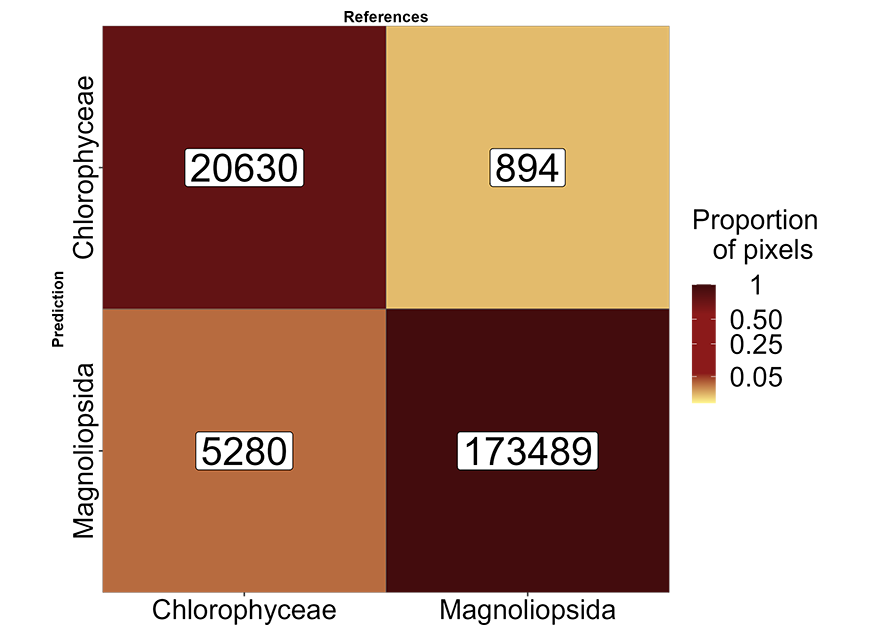
\includegraphics[width=1\textwidth,height=\textheight]{./Figures/Low_res/Validation/ConfusionMatrixGreen.png}

}

\caption{\label{fig-ValidationGreen}Sample of
Figure~\ref{fig-Validation} focusing on green macrophytes. The labels
inside the matrice indicate the number of pixels.}

\end{figure}%

The Micasense RedEdge-MX DUAL camera used in this study meets these two
criteria, enabling the classifier to achieve 97\% of accuracy between
these two classes (Figure~\ref{fig-ValidationGreen}). Even if the
pigment compostion of green macrophytes is similar, differences in the
spectral shape can still be observed (Figure~\ref{fig-vegetation}).
Several factors can explain these differences such has different pigment
concentration or proportion, different cellular organisation and 3D
disposition of the plant a whole on the intertidal mudflat
\citep[\citep{kirk1994light},
\citep{hedley2018influence}]{beach1997vivo}.

The VIP analysis of the Neural Network model (Figure~\ref{fig-VIP})
shows that the 531 nm band is the most important spectral band for
accurately identifying Chlorophyceae. In fact, at this wavelength,
Chlorophyceae exhibits the highest reflectance among all other classes,
highlighting the difference in accessories carotenoid proportion between
seagrasses and green algae \citep{repolho2017seagrass}.

Concerning Phaeophyceae, the thick cell walls of plant of this class
make it really reflective in the infrared part of the spectra whereas
the presence of Fucoxanthin and Zeaxanthin result in a low reflectance
in the visible part of the electromagnetic spectra. These two key
features has been identified by the Neural Network as the two principal
predictors to accurately identify Brown algae (Figure~\ref{fig-VIP}).
Similarly, the presence of phycoerythrin and phycocyanin in Rhodophyceae
contributes to the lowest reflectance among all classes in the spectral
range of 560 to 615 nm (Figure~\ref{fig-VIP}). The band at 560 nm has
been identified as important for accurately identifying this class
Resolution impact on the prediction. Regarding Bacillariophyceae, the
VIP analysis (Figure~\ref{fig-VIP}) indicates that 475 nm is the most
important predictor for this class. This could be attributed to the
absence of lutein, neoxanthin, and zeaxanthin in diatoms, absorbing in
the blue part of spectra, resulting in the highest visible reflectance
among all classes. Furethemore, it is vegetation with the lowest
concentration of chlorphyll-a, pigment absorbing light both in the blue
and the red. The transparency of Bacillariophyceae makes the reflectance
of the sediment part of the overall reflectance of Bacillariophyceae,
further explaining the high reflectance in the blue.

\subsection{Spectral Spatial Temporal Resolution impact on the
prediction}\label{spectral-spatial-temporal-resolution-impact-on-the-prediction}

\phantomsection\label{cell-fig-CompareRef}
\begin{figure}[H]

\centering{

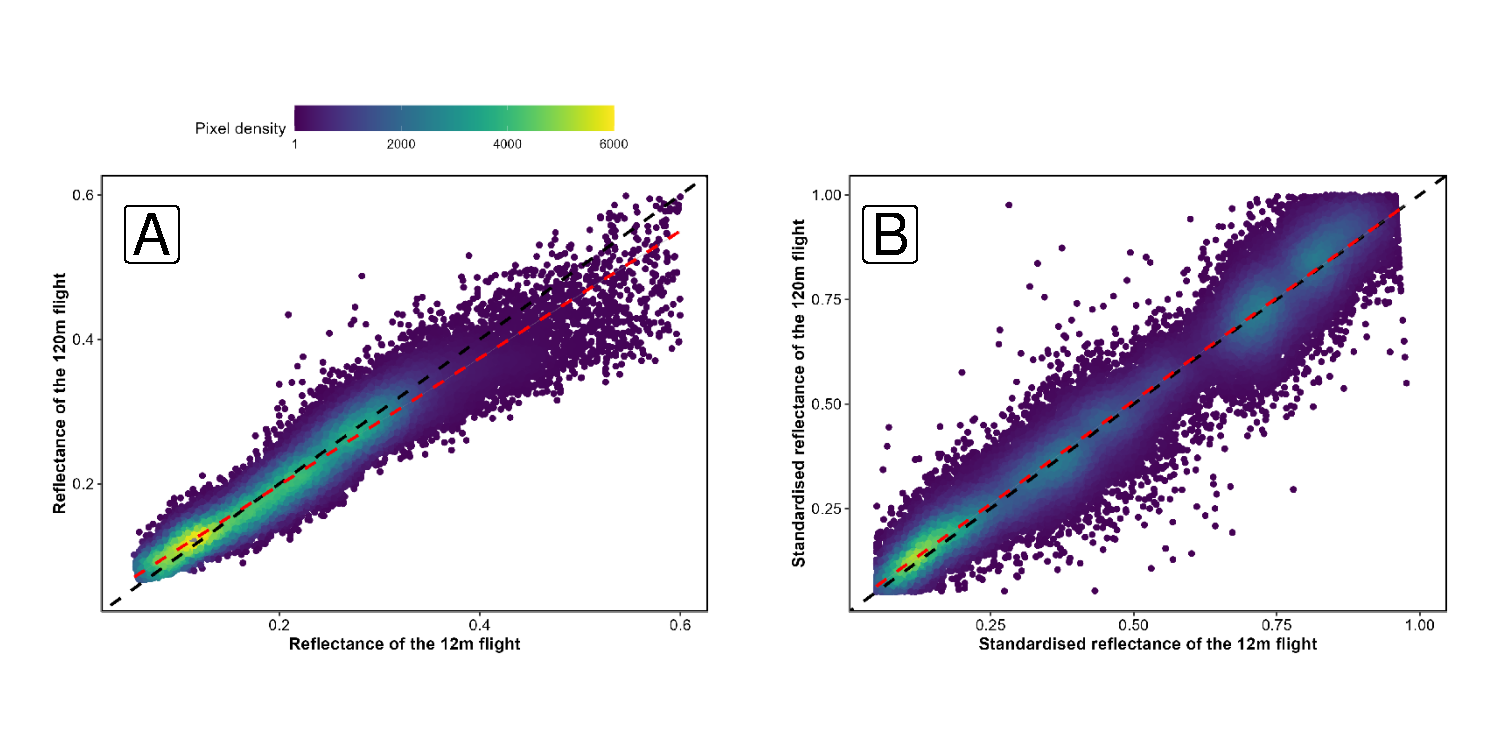
\includegraphics[width=1\textwidth,height=\textheight]{index_files/figure-pdf/fig-CompareRef-1.pdf}

}

\caption{\label{fig-CompareRef}Comparison of reflectance retrieved from
both low-altitude and high-altitude flights over a common area. The red
dashed line represents a linear model wheras the black dashed line
represents a 1 to 1 relationship. Left (A) plots RAW data and right (B)
plots standardise data.}

\end{figure}%

In this study, a key innovation lies in the utilization of two different
altitudes (12m and 120m) for constructing the neural network model. The
lower altitude flights (8mm spatial resolution) enable precise selection
of pure pixels representing the classes used in the neural network
model. This methodology implies a consistency between the reflectance of
both altitude. Figure~\ref{fig-CompareRef} (A) depicts the relationship
between reflectance from a low-altitude flight and a high-altitude
flight conducted over the same area. An apparent underestimation of
reflectance values is observed in the high-altitude flight, particularly
for higher values. Since both flights were conducted over vegetation
areas, the highest reflectance values correspond to the infrared part of
the spectrum.

The disparity in infrared reflectance may stem from temporal differences
between the flights, possibly resulting in a slightly drier intertidal
area and consequently higher infrared reflectance. This disparity poses
an issue for the methodology followed in the present study, relying
solely on one flight height for training. To address this issue, we
employed min/max standardized reflectance spectra as predictors for the
model (Equation~\ref{eq-std} ; Figure~\ref{fig-CompareRef} (B) ;
\citep{Cao2017}). This approach allows us to eliminate differences in
the level of reflectance, focusing instead on the shape of the spectra.
This is a key feature in building a model that can reliably predict
vegetation across geographical sites and seasons. It enables consistent
prediction of vegetation classes across variations in biomass and
variability in light conditions \citetext{\citealp[
]{fyfe2003spatial}; \citealp[
]{COSTA2021107018}; \citealp{piaser2023impact}}.

The Figure~\ref{fig-upscaling} demonstrates that a seagrass cover
percentage of 90 \% is necessary for confident prediction of seagrass
presence. This highlights a limitation of the methodology used to
construct the training dataset for the model. The dataset was composed
exclusively of pure pixels, which has resulted in the model's reduced
confidence when faced with lower percentages of seagrass cover.
Intertidal seagrasses exhibit strong phenology, with varying pigment
composition throughout the year\citetext{\citealp[
]{bargain2013seasonal}; \citealp{legare2022remote}}. This suggests that
outside of the biomass peak of seagrasses, this model may be less
accurate. Further investigation is warranted to explore this aspect.

\subsection{Application of the model}\label{application-of-the-model}

Climate change, global warming, alien and invasive species development,
coastal erosion, sealevel rise, while further impact coastal ecosystems
in the future \citetext{\citealp{SCHIBALSKI2022101414}; \citealp[
]{holon2018predictive}; \citealp{marquet2024global}}. The demand for
meaningful and efficient monitoring methods for these habitats has
therefore never been greater \citetext{\citealp[
]{muller2018satellite}; \citealp[
]{villalobos2023remote}; \citealp{oiry2021using}}. Our findings,
particularly the improved discrimination of vegetation types, underscore
the potential of drone-based remote sensing to support diverse
applications, from biodiversity conservation to climate change
adaptation strategies\textbf{.} Employing traditional sampling methods
to monitor these ecosystems is time and resource-intensive, and the
findings are often difficult to scale up. Earth observation methods can
bridge this gap and meet the needs for monitoring coastal ecosystems.
\citep{papathanasopoulou2019satellite}. The retrieval of Essential
Biodiversity Variables (EBVs) and Essential Ocean Variables (EOVs)
through satellite observations is increasingly common, enabling
comprehensive monitoring of entire ecosystems over extended time periods
\citetext{\citealp[
]{ratnarajah2023monitoring}; \citealp{ZOFFOLI2020112020}}. The
significance of monitoring waters, particularly in light of the Water
Framework Directive (WFD ; \citep{WFD2000}), cannot be overstated in
environmental management and conservation efforts. The WFD mandates the
achievement and maintenance of ``good ecological status'' for all
European waters, which necessitates a comprehensive understanding and
monitoring of aquatic ecosystems, including coastal habitats like
seagrass \citetext{\citealp[ ]{foden2007angiosperms}; \citealp[
]{nordlund2024one}; \citealp{Zoffoli2021}}.

Effective and efficient monitoring tools are essential for identifying
the impacts of human activities and natural changes on these ecosystems.
Drones, with their capability for high-resolution, multispectral
imagery, provide a novel and powerful means to rapidly and accurately
acquire ground truth data (i.e.~output of the model used in the present
study). This data is critical for calibrating and validating satellite
remote sensing applications, thereby enhancing our capacity to monitor
vast coastal areas systematically under the WFD framework. The
integration of drone technology facilitates a scalable approach to
environmental surveillance, offering significant advancements in the
spatial and temporal resolution of data collection. This, in turn,
supports the directive's objectives by enabling more informed and timely
management decisions for the preservation and restoration of aquatic
ecosystems.

\section{Conclusion}\label{conclusion}

The utilization of drone-based remote sensing coupled with machine
learning techniques has proven to be an effective method for the
discrimination of seagrasses and macroalgae in coastal ecosystems. This
study has highlighted the potential for these technologies to enhance
the accuracy and efficiency of habitat monitoring, which is essential
for environmental management and conservation strategies. Through the
application of high-resolution multispectral imagery, the research
contributes to the broader understanding and surveillance of aquatic
ecosystems, aligning with objectives outlined in policies such as the
Water Framework Directive. The findings underscore the importance of
adopting advanced remote sensing tools in ecological studies and
environmental monitoring, providing a foundation for future research and
policy implementation aimed at ecosystem preservation and restoration.


  \bibliography{library.bib}


\end{document}
